% \documentclass[12pt]{mitthesis}
% \usepackage[pdftex]{graphicx}
% \usepackage{subfloat}
% \usepackage{kylesthesis}
% \begin{document}

% \tableofcontents
% \clearpage

% %\listoffigures
% %\clearpage

% \subsubsection*{NOTES}
% \clearpage

% \setcounter{chapter}{5}
\chapter{  IR-UV double resonance LIF/SEELEM spectroscopy of the
  $3^34^1$ \Ka{0} and $3^36^1$ \Ka{0} vibrational sublevels of $S_1$
  acetylene}

\section{Introduction}

The \AtoX\ spectrum of acetylene, \ce{C2H2}, provides a paradigm for
an electronic transition accompanied by a change in geometry.  The
acetylene molecule is linear in the ground state ($S_0$), but has a
planar \emph{trans}-bent geometry in the \astate\ state ($S_1$)
\cite{king52, ingold53, innes54}.  \emph{Ab initio} calculations are
in agreement that all low-lying electronic excited states, singlet and
triplet, have minima in a planar \emph{trans}-bent geometry
\cite{demoulin75, lischka86, yamaguchi93, sherrill96, malsch98,
  ventura03}.  The sole exception is the third triplet state, $T_3$,
which instead has a minimum in a non-planar geometry, twisted
approximately 75\degrees\ out of plane from the \emph{trans}
configuration \cite{cui96, ventura03, thom07}.

Experiment and theory have shown that vibrational levels of the $T_3$
electronic state play a crucial role in allowing mixing between $S_1$
levels and the dense manifold of optically dark $T_{1,2}$ levels
\cite{humphrey97, altunata00, dupre93, cui97, thom07, ventura03}.  The
fundamental premise of the model is that spin-orbit matrix elements
between $S_1$ and $T_{1,2}$ levels are much smaller than those between
levels of $T_3$ and $T_{1,2}$.  In the doorway model, mixing between
$S_1$ and $T_{1,2}$ levels occurs as a second-order effect; a level
of $S_1$ must mix with $T_3$, which, in turn, permits mixing with the
manifold of $T_{1,2}$ levels.

% The word ``doorway'' implies that the $S_1 \sim T_3$ mixing is
% dominated by a single $T_3$ vibrational level.  Because the levels of
% $T_3$ are so widely spaced ($\sim 10$ \rcm) relative to the average
% $S_1 \sim T_3$ spin-orbit matrix element ($\sim 0.1$ \rcm), this is
% almost always the case.

The magnitude of $S_1 \sim T_3$ spin-orbit matrix elements is
controlled principally by vibrational overlap factors, resulting in
vibrational specificity for $S_1 \sim T_3$ mixing.  To date, most
studies have addressed the role of the symmetric \emph{trans}-bending
mode, partially because the levels containing this
Franck-Condon-active vibration are well understood and appear with
great intensity in the \AtoX\ spectrum.  Many studies have observed an
increase in $T_3$-mediated $S_1 \sim T_{1,2}$ mixing with increased
excitation in the $\nu_3$ (\emph{trans}-bend) vibrational mode of
\astate\ acetylene \cite{dupre91, ochi91, humphrey97}.

The role of the non-symmetric bending modes, $\nu_4$ (torsion) and
$\nu_6$ (antisymmetric in-plane bend), is much less clear.  Since the
geometry change from in-plane to out-of-plane occurs along the
torsional coordinate, a simple Franck-Condon model would predict that
increased excitation in the torsional mode ($\nu_4$) would lead to
increased $S_1 \sim T_3$ vibrational overlap.  However, the current
experimental evidence and theoretical calculations disagree with this
na\"{i}ve model.  Mizoguchi et al. observe large splittings in the
spectrum of $3^36^1$ \Ka{1}, but not in the spectrum of $3^34^1$
\Ka{1} \cite{mizoguchi00}.  Yamakita and coworkers observe Zeeman
quantum beats in several rotational lines in the spectrum of $3^36^1$
\Ka{1}, but none in the spectrum of $3^34^1$ \Ka{1} \cite{yamakita01}.
These authors cite agreement with the calculations of Cui and
Morokuma, who predict a half-linear geometry for the minimum of the
seam of intersection between the $S_1$ and $T_3$ electronic surfaces
\cite{cui96}.  Such a half-linear geometry is accessible via a
combination of the $\nu_3$ and $\nu_6$ vibrations.

We are left without explanation as to the small magnitude vibrational
overlap integrals upon excitation in mode 4, relative to mode 6.  In
an effort to address this problem, Virgo and coworkers recently
published a comparison of the simultaneously recorded SEELEM/LIF
spectrum of the $2^13^14^2$ \Ka{1} and $2^13^16^2$ \Ka{1} sublevels.
They observe that the SEELEM:LIF intensity ratio is three times larger
for $2^13^14^2$ \Ka{1} than for $2^13^16^2$ \Ka{1}.  In order to
characterize the experimental results in terms of $2^13^14^2$ and
$2^13^16^2$ basis character, they present a tentative deperturbation
of the $2^13^1B^2$ polyad, which consists of the $2^13^14^2$ ($a_g$),
$2^13^16^2$ ($a_g$), and $2^13^14^16^1$ ($b_g$) levels.  They
determine that $2^13^14^2$ and $2^13^16^2$ basis character is
essentially evenly distributed between the two \Ka{1} sublevels
observed in the experiment.  The difference in SEELEM:LIF intensity
ratio is ascribed instead to be the result of an interference effect
which cancels out almost all $2^13^14^16^1$ ($b_g$) basis character in
one of the levels.

The interference effect is due to two separate, strong interactions
between the $\nu_4$ and $\nu_6$ vibrations.  The first interaction is
a strong Darling-Dennison resonance, which connects vibrations by
exchanging two quanta of $\nu_4$ for two quanta of $\nu_6$, or vice
versa.  Levels with only one quantum of modes 4 or 6, such as those
studied by Mizoguchi, are immune to this effect.  The second
interaction is the $a$-axis Coriolis coupling, which exchanges one
quantum of mode 4 for one quantum of mode 6.  The matrix element for
$a$-axis Coriolis coupling includes a factor of $K$, thus sublevels
with $K=0$ are immune to this effect.

In this study, we seek to address the role of modes 4 and 6 in
promoting vibrational overlap with $T_3$ levels.  To avoid the
Darling-Dennison resonance, we select a polyad with one quantum of
non-symmetric bend.  To avoid \emph{a}-type Coriolis coupling, we examine
the $K=0$ sublevels of the polyad members.  To investigate the effects
of $\nu_4$ and $\nu_6$ near the crucial half-linear and twisted
geometries, we select the particular combination levels $3^34^1$ and
$3^36^1$ of $S_1$ acetylene.





























\section{Experiment}

Vibrational levels of \astate\ acetylene with \emph{ungerade}
symmetry are inaccessible via one-photon transitions from the ground
state, according to $g$/$u$ selection rules.  To access the $3^34^1$
($a_u$) and $3^36^1$ ($b_u$) levels, we employed an IR-UV double
resonance scheme.  The $\nu_3''+\nu_4''$ level of the \xstate\ state
was chosen as an intermediate state for laser excitation.  According
to the selection rule $K'-\ell'' = \pm 1$, the $K'=0$ sublevels of
$3^34^1$ and $3^36^1$ are accessible from this $\ell''=1$ ground state
intermediate.

IR laser radiation in the region of 3900 \rcm\ was generated by a
method of difference frequency mixing (DFM) followed by optical
parametric amplification (OPA).  The second harmonic output of an
injection-seeded Nd:YAG laser (Spectra Physics PRO-270) was used to
pump a tunable dye laser (Lambda Physik FL2002), operating with LDS
751 laser dye.  The dye laser output was mixed in a lithium niobate
(\ce{LiNbO3}) crystal with a portion of the 1064 nm Nd:YAG fundamental
beam.  The IR output was amplified in another \ce{LiNbO3} crystal,
using the remaining 1064 nm radiation.  The amplified IR laser
radiation had a typical power of 3 mJ and an incoherent linewidth of
0.15 \rcm.  A photoacoustic cell containing approximately 100 mTorr of
acetylene was used for calibration of the IR radiation.

The UV laser radiation used in the second step of the double resonance
was generated from the output of a second dye laser (Lambda Physik
FL3002), operating with Coumarin 480, pumped by the third harmonic of
the Nd:YAG laser described above.  The dye laser output was frequency
doubled using a BBO crystal.  The UV laser radiation was calibrated by
recording the absorption spectrum of \ce{^{130}Te2} using the fundamental
frequency output of the dye laser.  The frequency step size of the UV
laser was approximately 0.047 \rcm\ (frequency doubled output) in this
study.

The IR and UV beams were positioned in an overlapping, colinear
geometry inside the SEELEM/LIF apparatus.  The UV laser pulse was
delayed by 10 ns relative to the IR pulse by using several UV
reflectors to create an optical delay line.  A dichroic mirror,
transparent in the IR, was used to combine the IR and UV beams.
Except where noted, both beams were $p$-polarized, relative to the
plane defined by the direction of laser propogation and the molecular
beam axis of the apparatus.

The SEELEM/LIF apparatus, in its current arrangement, has been
described previously \cite{cunningham-thesis, altunata-thesis,
  altunata02, mishra04}.  Briefly, the apparatus consists
of two differentially pumped vacuum chambers, a source chamber and a
SEELEM detection chamber.  In the source chamber, a supersonic jet of
acetylene gas (Matheson) is expanded from a 10 Hz pulsed valve
(Jordan).  The source chamber is pumped by a 6 inch diffusion pump
(Varian), and has a typical operating pressure of $10^{-4}$ Torr.
Approximately 2 cm downstream from the nozzle, the molecules are
excited by the overlapping UV and IR laser beams, which intersect the
axis of the jet at a 90\degrees\ angle.  The laser-induced molecular
fluorescence is collected by $f/4$ optics along an axis normal to the
plane defined by the lasers and the jet axis.  The fluorescence passes
through a filter (UG-11) and is detected by a photomultiplier tube
(Hamamatsu R375).  The time-varying photomultiplier output signal is
averaged at each laser frequency on a digital oscilloscope (LeCroy)
and recorded on a PC %\TODO{Determine how many bits the scope has}.

Approximately 5 cm from the region of excitation, molecules in the
supersonic expansion pass through a 3 mm diameter skimmer and enter
the SEELEM detection chamber.  The detection chamber is also pumped by
a 6 inch diffusion pump (Varian), and has a typical operating pressure
of $10^{-6}$ Torr.  The SEELEM detector is positioned along the
molecular beam axis, approximately 35 cm downstream of the excitation
region.  The design of the SEELEM detector used in these experiments
has been described by several authors \cite{cunningham-thesis,
  altunata-thesis}.  In the SEELEM detector, electrons
ejected from a grounded metal surface are detected by an electron
multiplier (ETP).  The electron multiplier output is sent to a fast
amplifier/discriminator (EG\&G/Ortec), and the resulting pulses are
acquired by PC-operated multichannel scalar hardware.

To eject an electron from the metal surface of the SEELEM detector, an
excited molecule must have a vertical electronic excitation energy
exceeding the work function of the metal.  In this study, a gold
surface was used, with a work function of approximately 5.1 eV.
Among the low-lying electronically excited states of acetylene, only
$S_1$ and $T_3$ have sufficient energy to be detectable on gold.





















\section{Results}

The spectra in this study were collected using two double resonance
strategies: a survey method and an ``individual line'' method.  In the
survey method, the IR laser was tuned to the Q-branch head of the
$\nu_3''+\nu_4''$ level in the ground electronic state.  The Q-branch of
this band is very compact, and the incoherent linewidth of the IR
laser is sufficient to excite the rotational levels $J=1f-5f$ at a
single laser frequency.  From the $f$-symmetry rotational levels
populated in the first excitation step, Q-branch transitions in the UV
are permitted to the $3^34^1$ \Ka{0} sublevel, and P or R-branch
transitions are permitted to the $3^36^1$ \Ka{0} sublevel.  A diagram
of the energy levels and the allowed transitions is shown in Figure
\ref{fig:levels-iruvdr}.

\begin{figure}
  \centering
  
  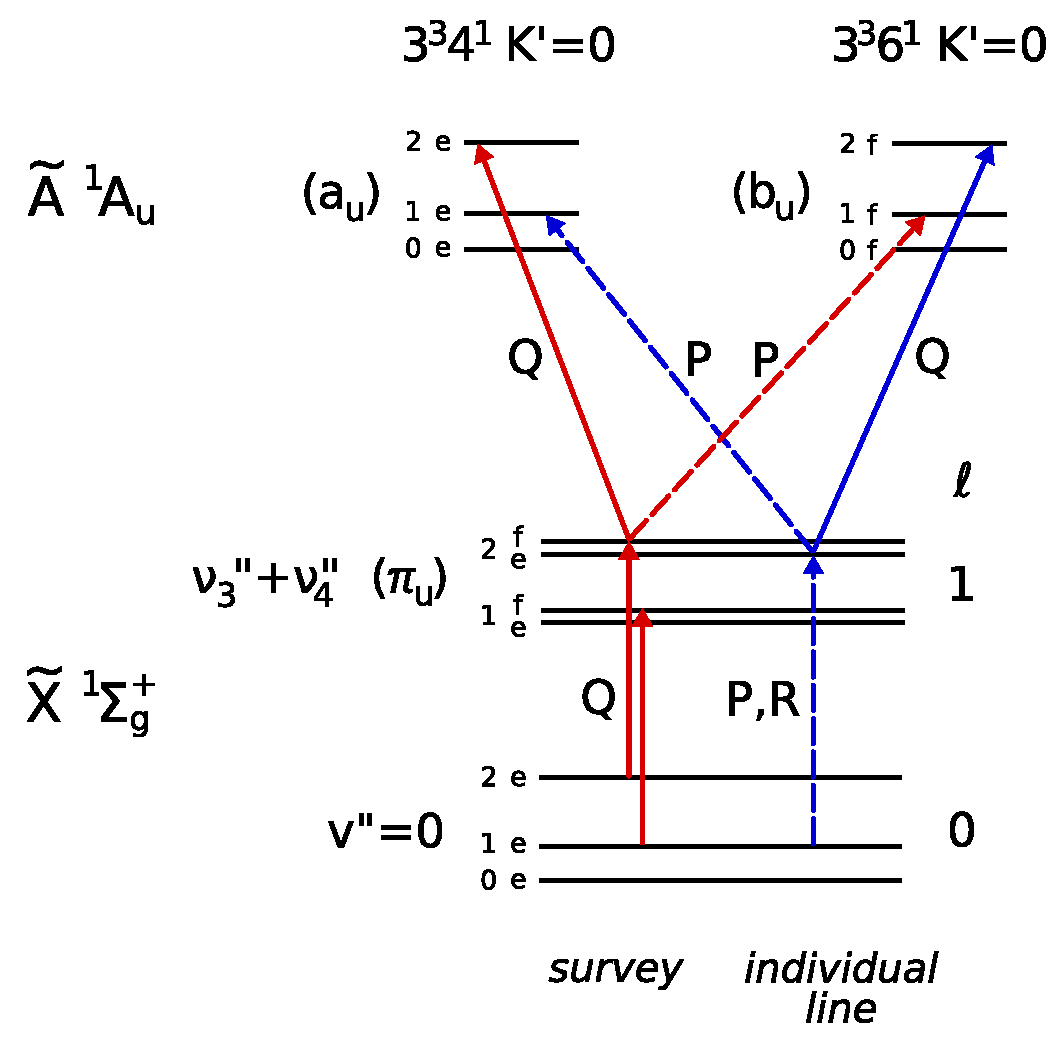
\includegraphics[width=5in]{levels-iruvdr}

  \caption{Schematic diagram of the IR-UV double resonance methods
    used in this study.  In the survey method, the Q(1)-Q(5)
    transitions terminating in the $\nu_3''+\nu_4''$ level of the
    ground state are pumped at a single IR laser frequency.  From the
    populated $f$-symmetry rotational levels, Q-branch transitions in
    the UV are permitted to the $3^34^1$ \Ka{0} sublevel, and P or
    R-branch transitions are permitted to the $3^36^1$ \Ka{0}
    sublevel.  In the individual line method, a single P or R-branch
    transition is excited in the ground state.  In this case,
    $e$-symmetry levels of $\nu_3''+\nu_4''$ are excited by the IR
    laser, and the selection rules for P, R vs. Q branches in the UV
    are reversed.}
  \label{fig:levels-iruvdr}
\end{figure}

In the individual line method, the IR laser was tuned to individual line
transitions in the P or R-branch of the $\nu_3''+\nu_4''$ level in the
ground electronic state.  Using this strategy, only a single
$e$-symmetry rotational level of $\nu_3''+\nu_4''$ is populated by the
IR laser at a given frequency.  From the intermediate state, only a
single Q-branch transition to the $3^36^1$ \Ka{0} sublevel of the
\astate\ state is permitted in the UV.  The $3^34^1$ \Ka{0} sublevel
of the \astate\ state is accessible through P or R-branch transitions
from the intermediate state, as shown in Figure
\ref{fig:levels-iruvdr}.


Figures \ref{fig:3361-q1}--\ref{fig:3361-q5} show the simultaneously
recorded SEELEM (plotted upward) and LIF (plotted downward) spectra of
the $J'=1-5$ rotational levels of \astate\ $3^36^1$ \Ka{1}, recorded
using the individual line method.  The SEELEM:LIF intensity ratio was on
the same order of magnitude as that of the $3^3$ \Ka{1} sublevel,
reported previously \cite{mishra04}. Figures
\ref{fig:3361-q1}--\ref{fig:3361-q5} each contain a magnified view of
the SEELEM spectrum, showing a large number of transitions to
long-lived eigenstates over each energy range scanned by our UV laser.
Unlike previous experiments, each spectrum in Figures
\ref{fig:3361-q1}--\ref{fig:3361-q5} contains eigenstates belonging to only
one value of the rotational quantum number, $J'$.  Using the individual line
double resonance method, the full envelope of metastable eigenstates
drawing intensity from each singlet basis state is viewed without
overlap from neighboring $J'$ transitions.

The LIF spectra in Figures \ref{fig:3361-q1}--\ref{fig:3361-q5} are
integrated in two time regions: an early time window
($0.5\tau_s-2\tau_s$, solid trace) and a delayed time window
($10\tau_s-18\tau_s$, dashed trace).  The quantity $\tau_s$ is the
characteristic fluorescence lifetime of the \astate\ state,
determined to be 270 ns \cite{ochi91}.  Line splittings are resolved
in the early and delayed LIF spectra of the $J'=1-4$ rotational
levels.  The frequency separation of the components in the splittings
varies between 0.06 and 0.2 \rcm.  In each figure, the line with
greatest intensity in the early LIF spectrum is marked with a solid
indicator.  Additional lines, appearing with greater intensity in the
delayed LIF spectrum, are marked with dashed indicators.

In the spectra under consideration, all oscillator strength is
provided by a single, optically bright $S_1$ basis state.  Optically
dark basis states, triplet in character, may mix with the bright state
by spin-orbit interaction, according to the selection rule $\Delta J =
0$.  The fluorescence lifetime of the resultant eigenstates is
inversely proportional to the fractional $S_1$ electronic character,
as detailed in Chapter 4, Section 2.  The eigenstate that has the
largest amount of fractional $S_1$ character is labeled as the nominal
bright state.  This eigenstate has the shortest lifetime among the
ensemble of mixed eigenstates.  Levels with less fractional $S_1$
character have longer lifetimes and greater intensity in the delayed
LIF spectrum, relative to the early LIF spectrum.  Conequently, for
each spectrum we signify only the single highest-intensity line in the
early LIF channel with a solid marker, indicating its status as the
nominal bright state.

%%%%%%%%%%%%%%%%%%%%%%%%%%%%%%%%%%%%%%%%%%%%%%%%%%%%%%
%%
%% INSERT 3^3 6^1 INDIV FIGURES HERE
%%
%%%%%%%%%%%%%%%%%%%%%%%%%%%%%%%%%%%%%%%%%%%%%%%%%%%%%%

\begin{figure}
  \caption{Simultaneously recorded SEELEM (upper trace) and LIF (lower
    trace) spectra of the $3^36^1$ \Ka{0} sublevel of the \astate\
    state of \ce{C2H2}.  The P(2) line of the \xstate\ $\nu_3'' +
    \nu_4''$ level is used as an intermediate state in the experiment,
    so only the Q(1) line is observed in the upper state, according to
    Figure \ref{fig:levels-iruvdr}.  The LIF spectrum is integrated in
    two time regions: an early time window ($0.5\tau_s-2\tau_s$, solid
    trace) and a delayed time window ($10\tau_s-18\tau_s$, dashed
    trace).  Two additional lines, labeled with dashed markers, are
    observed in the delayed LIF spectrum on either side of the
    nominally singlet eigenstate. The intensity envelope of the
    delayed LIF spectrum closely resembles that of the SEELEM spectrum
    -- this effect appears throughout the subsequent figures.}
  \label{fig:3361-q1}
  \centering
  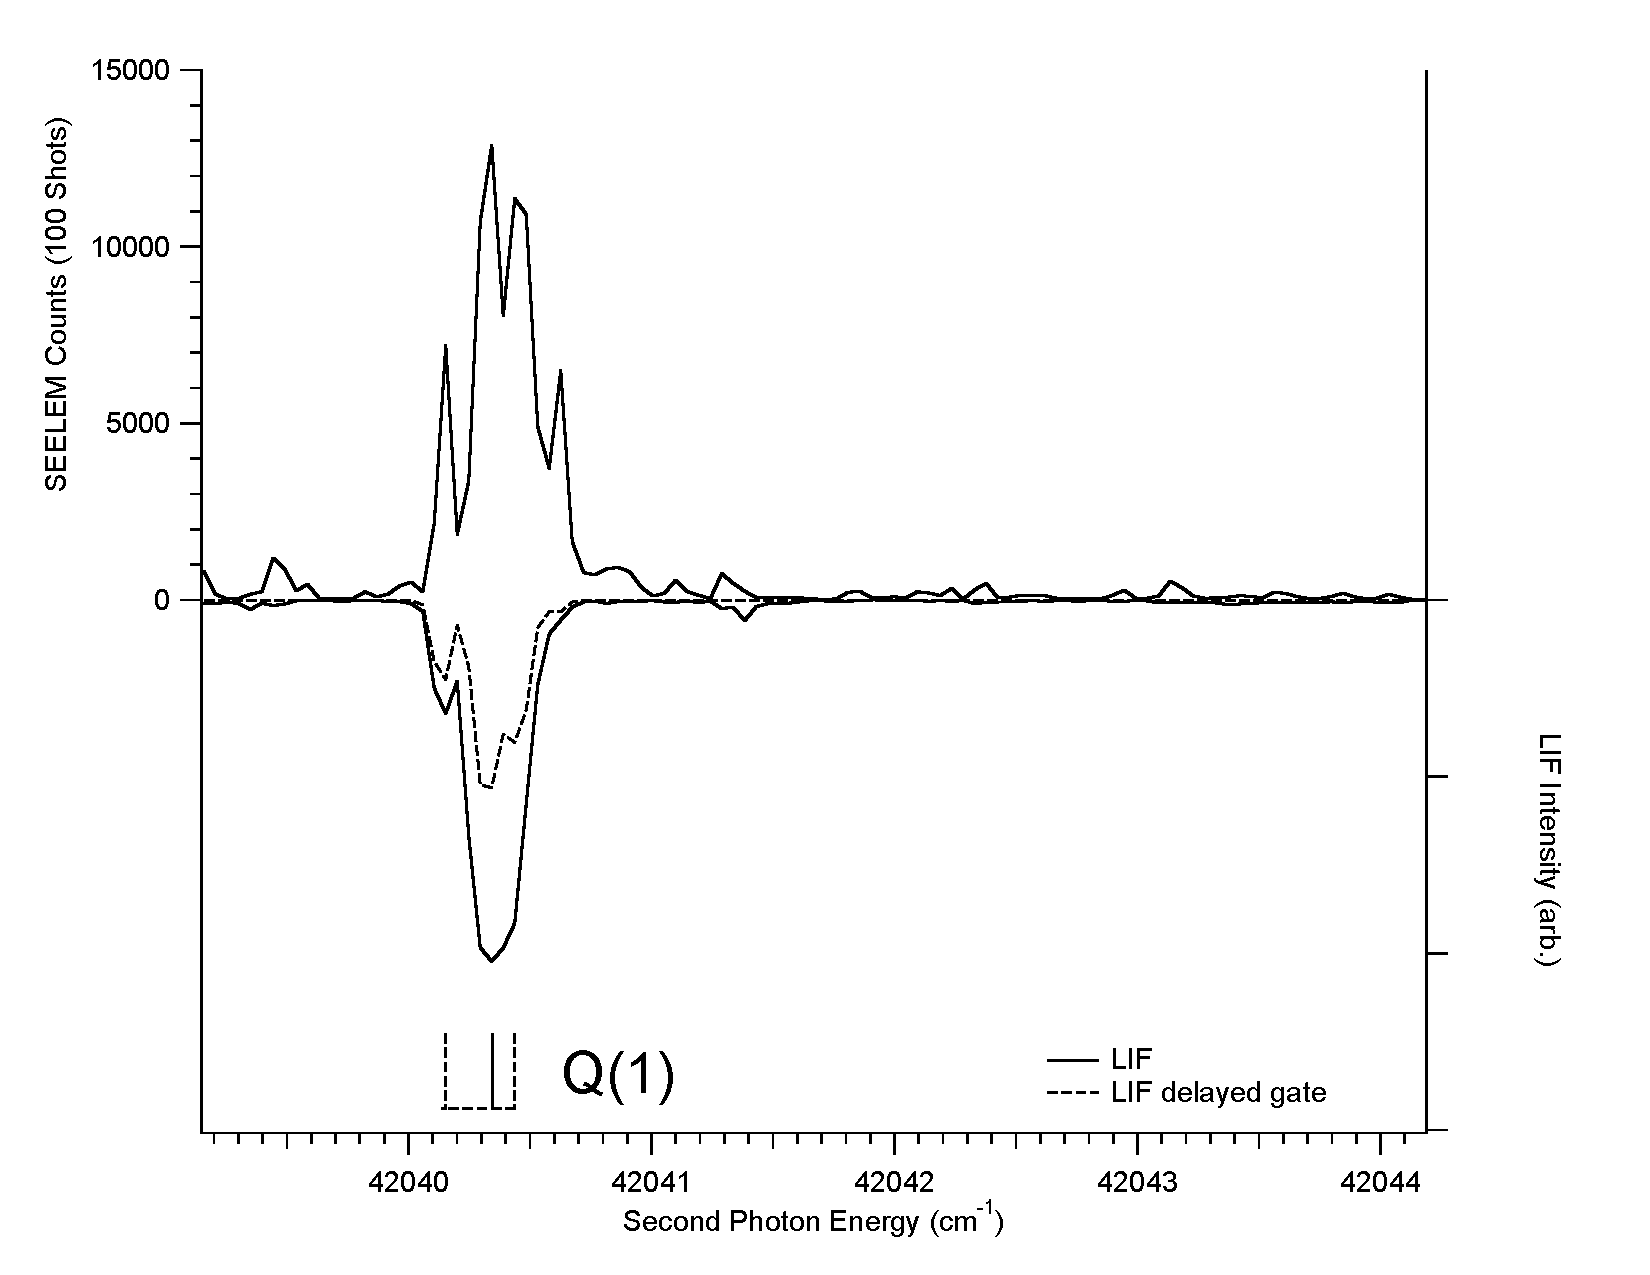
\includegraphics[width=6in]{spectrum-3361-q1-split.pdf}
  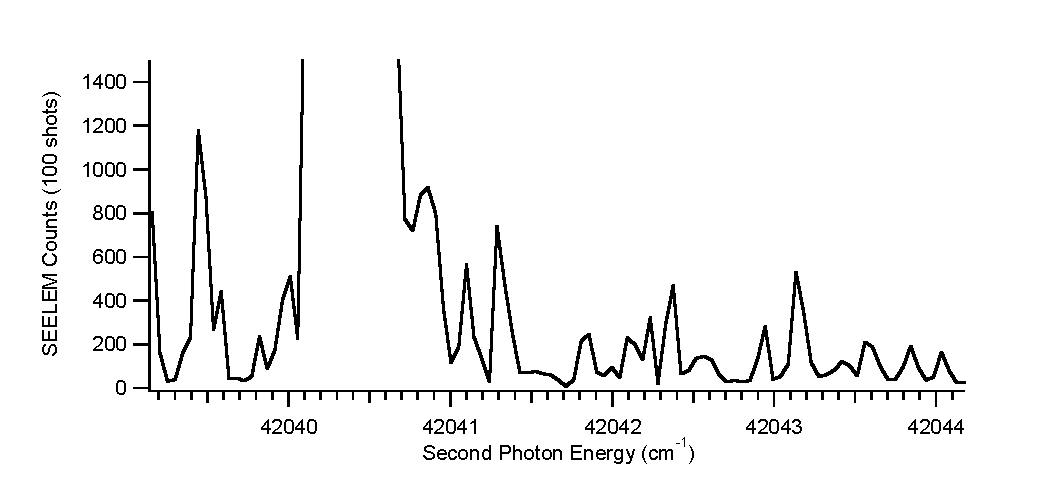
\includegraphics[width=5.5in]{spectrum-3361-q1-zoom.pdf}
\end{figure}

\begin{figure}
  \caption{Simultaneously recorded SEELEM (upper trace) and LIF (lower
    trace) spectra of the $3^36^1$ \Ka{0} sublevel of the \astate\
    state of \ce{C2H2}.  The P(3) line of the \xstate\ $\nu_3'' +
    \nu_4''$ level is used as an intermediate state in the experiment,
    so only the Q(2) line is observed in the upper state, according to
    Figure \ref{fig:levels-iruvdr}.  The LIF spectrum is integrated in
    two time regions: an early time window ($0.5\tau_s-2\tau_s$, solid
    trace) and a delayed time window ($10\tau_s-18\tau_s$, dashed
    trace).  A line splitting of $\sim 2$ \rcm\ is observed in the LIF
    spectrum, with the longer-lifetime (nominally triplet) component
    located at higher energy.}
  \label{fig:3361-q2}
  \centering
  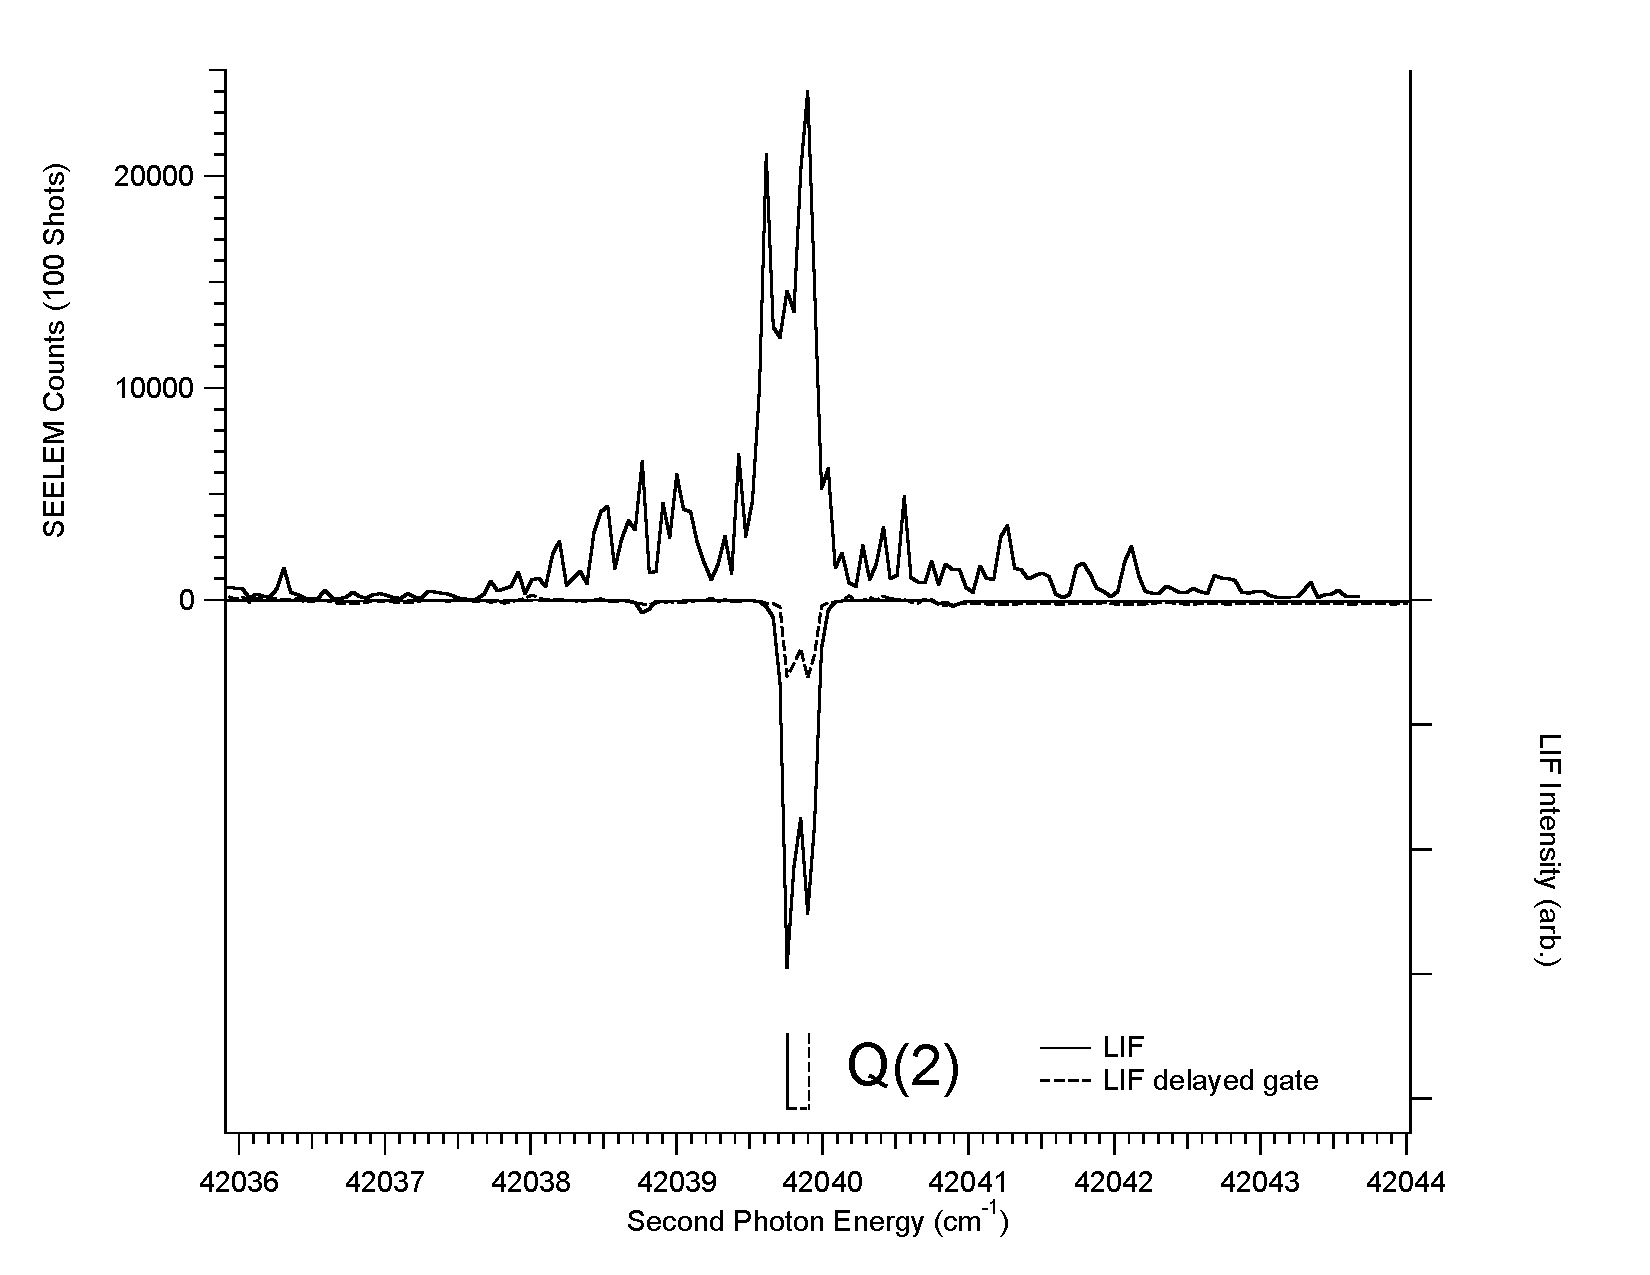
\includegraphics[width=6in]{spectrum-3361-q2-split.pdf}
  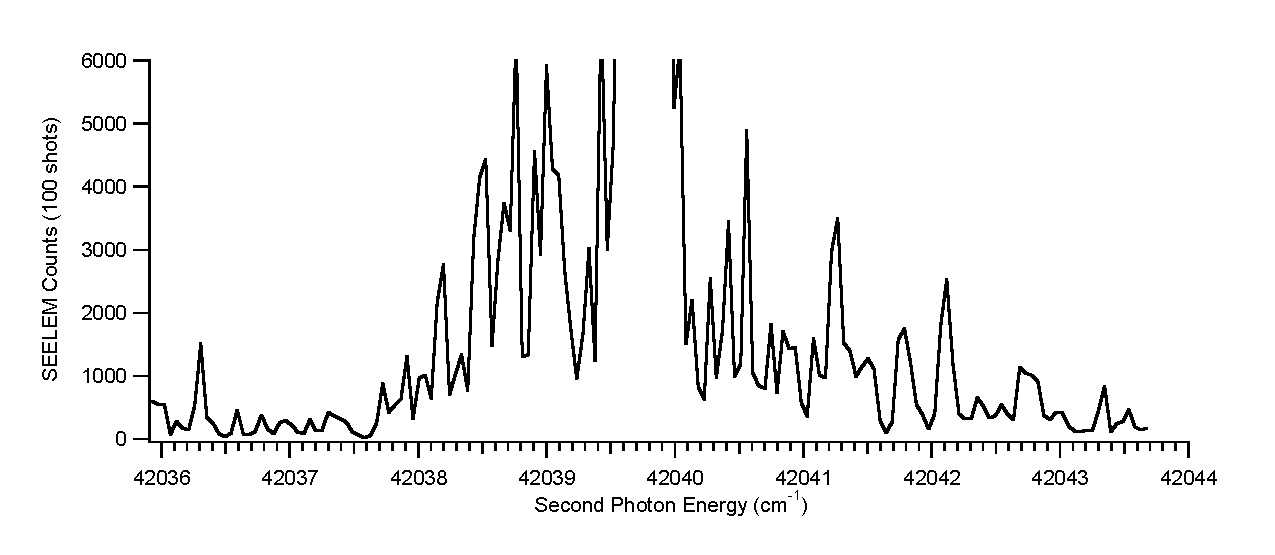
\includegraphics[width=6in]{spectrum-3361-q2-zoom.pdf}
\end{figure}

\begin{figure}
  \caption{Simultaneously recorded SEELEM (upper trace) and LIF (lower
    trace) spectra of the $3^36^1$ \Ka{0} sublevel of the \astate\
    state of \ce{C2H2}.  The P(4) line of the \xstate\ $\nu_3'' +
    \nu_4''$ level is used as an intermediate state in the experiment,
    so only the Q(3) line is observed in the upper state, according to
    Figure \ref{fig:levels-iruvdr}.  The LIF spectrum is integrated in
    two time regions: an early time window ($0.5\tau_s-2\tau_s$, solid
    trace) and a delayed time window ($10\tau_s-18\tau_s$, dashed
    trace).  The transition at 42038.3 \rcm\ has a short lifetime, and
    belongs to an unassigned singlet sublevel.  A small line splitting
    of less than $0.05$ \rcm\ is apparent from the shifted peak
    position in the delayed LIF spectrum relative to the early LIF
    spectrum.  The longer-lifetime (nominally triplet) component is
    located to higher energy.}
  \label{fig:3361-q3}
  \centering
  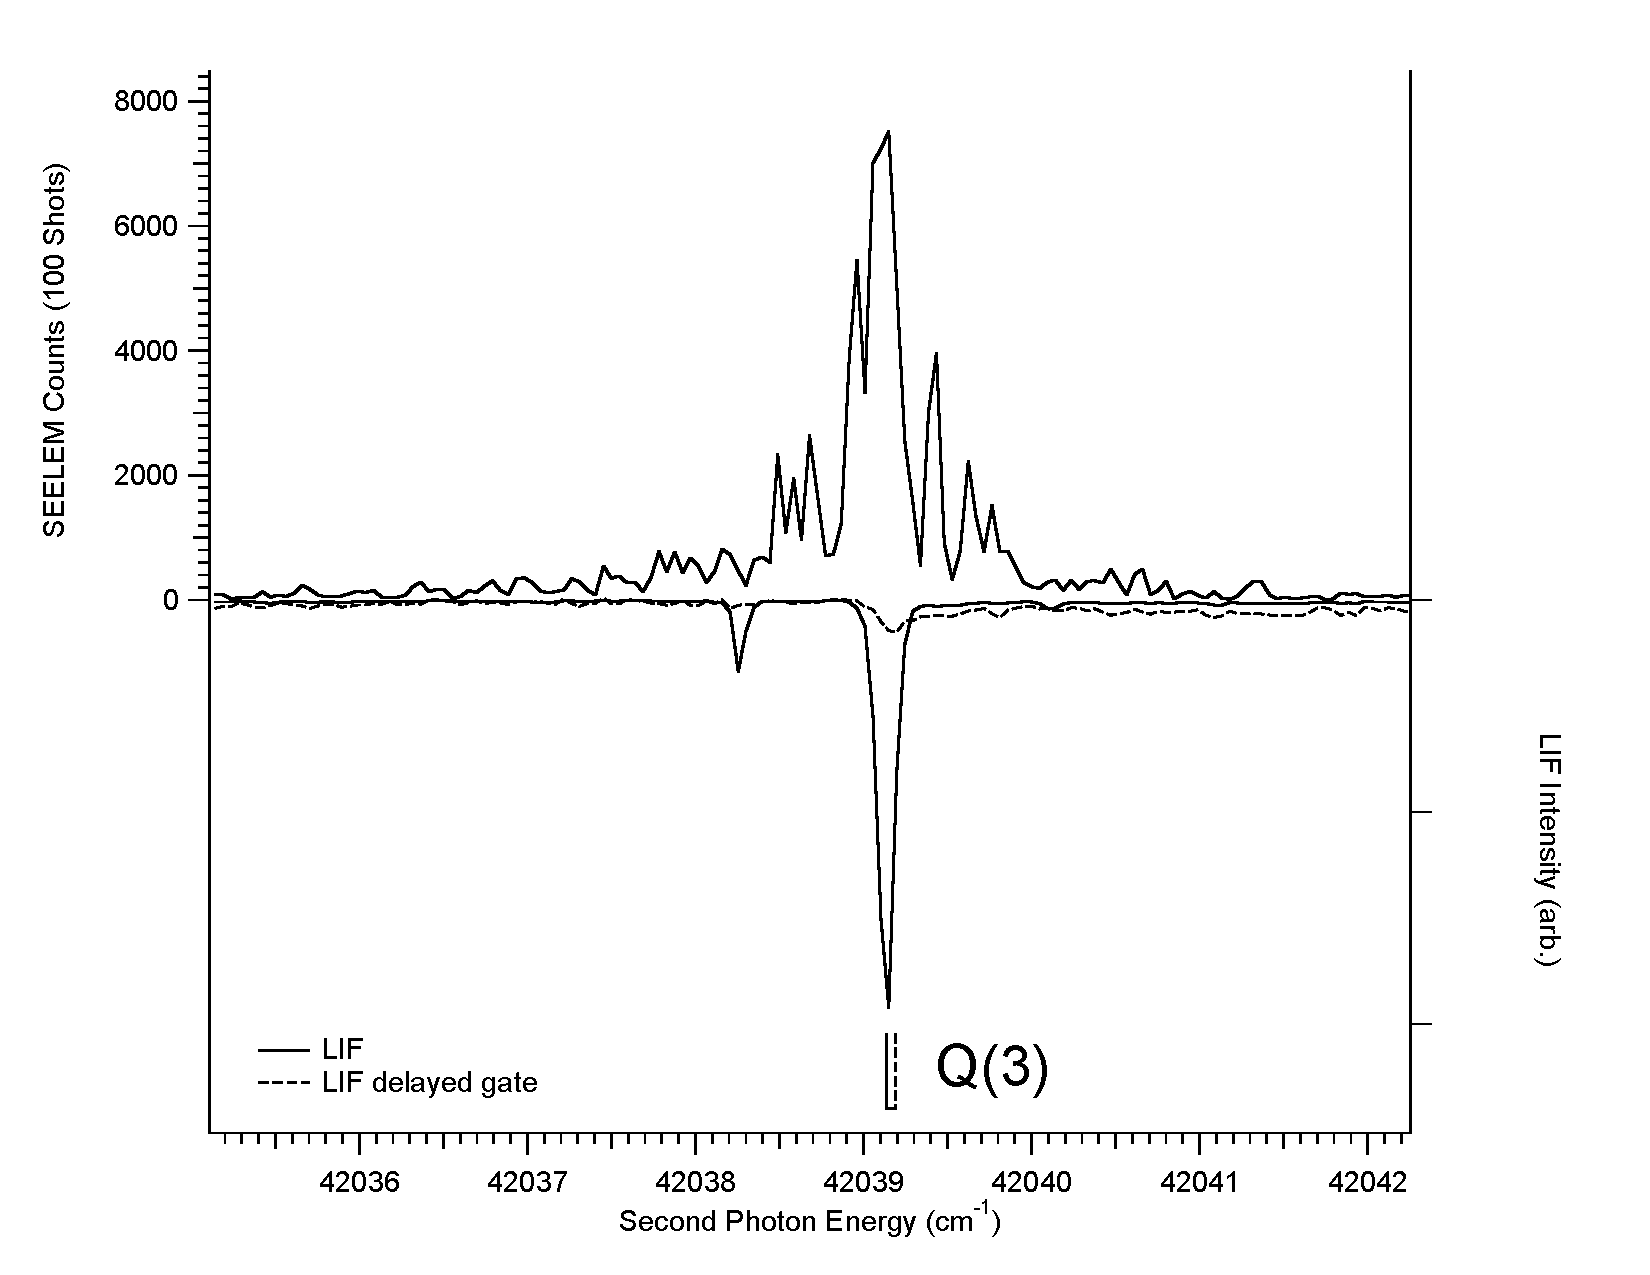
\includegraphics[width=6in]{spectrum-3361-q3-split.pdf}
  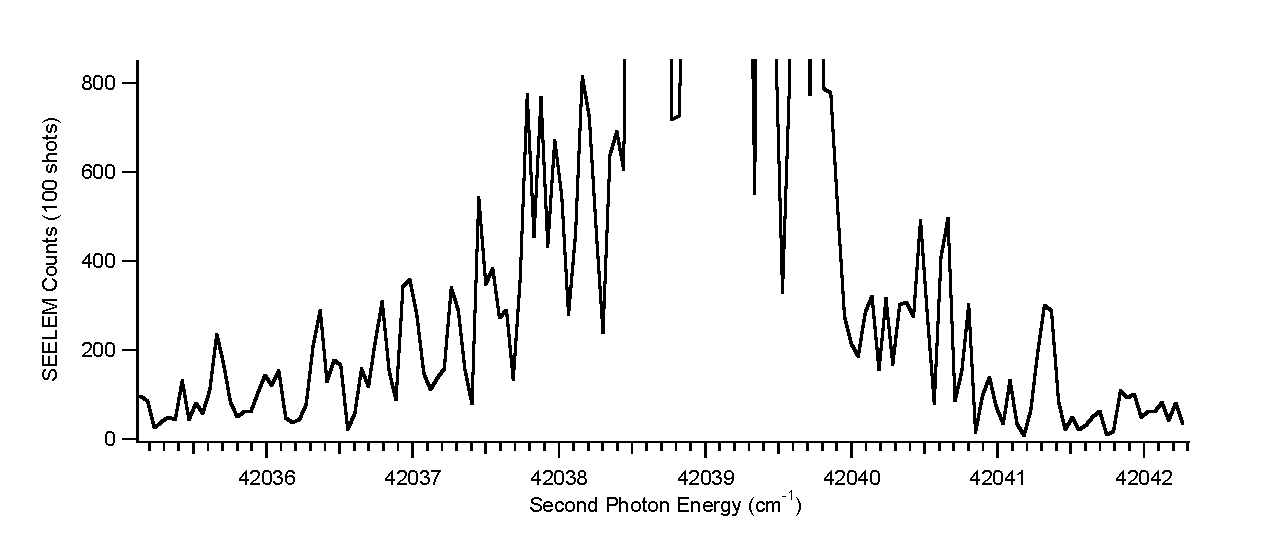
\includegraphics[width=6in]{spectrum-3361-q3-zoom.pdf}
\end{figure}

\begin{figure}
  \caption{Simultaneously recorded SEELEM (upper trace) and LIF (lower
    trace) spectra of the $3^36^1$ \Ka{0} sublevel of the \astate\
    state of \ce{C2H2}.  The R(3) line of the \xstate\ $\nu_3'' +
    \nu_4''$ level is used as an intermediate state in the experiment,
    so only the Q(4) line is observed in the upper state, according to
    Figure \ref{fig:levels-iruvdr}.  The LIF spectrum is integrated in
    two time regions: an early time window ($0.5\tau_s-2\tau_s$, solid
    trace) and a delayed time window ($10\tau_s-18\tau_s$, dashed
    trace).  A line splitting of $\sim0.2$ \rcm\ is observed in the LIF
    spectrum, with the longer-lifetime (nominally triplet) component
    located at higher energy.}
  \label{fig:3361-q4}
  \centering
  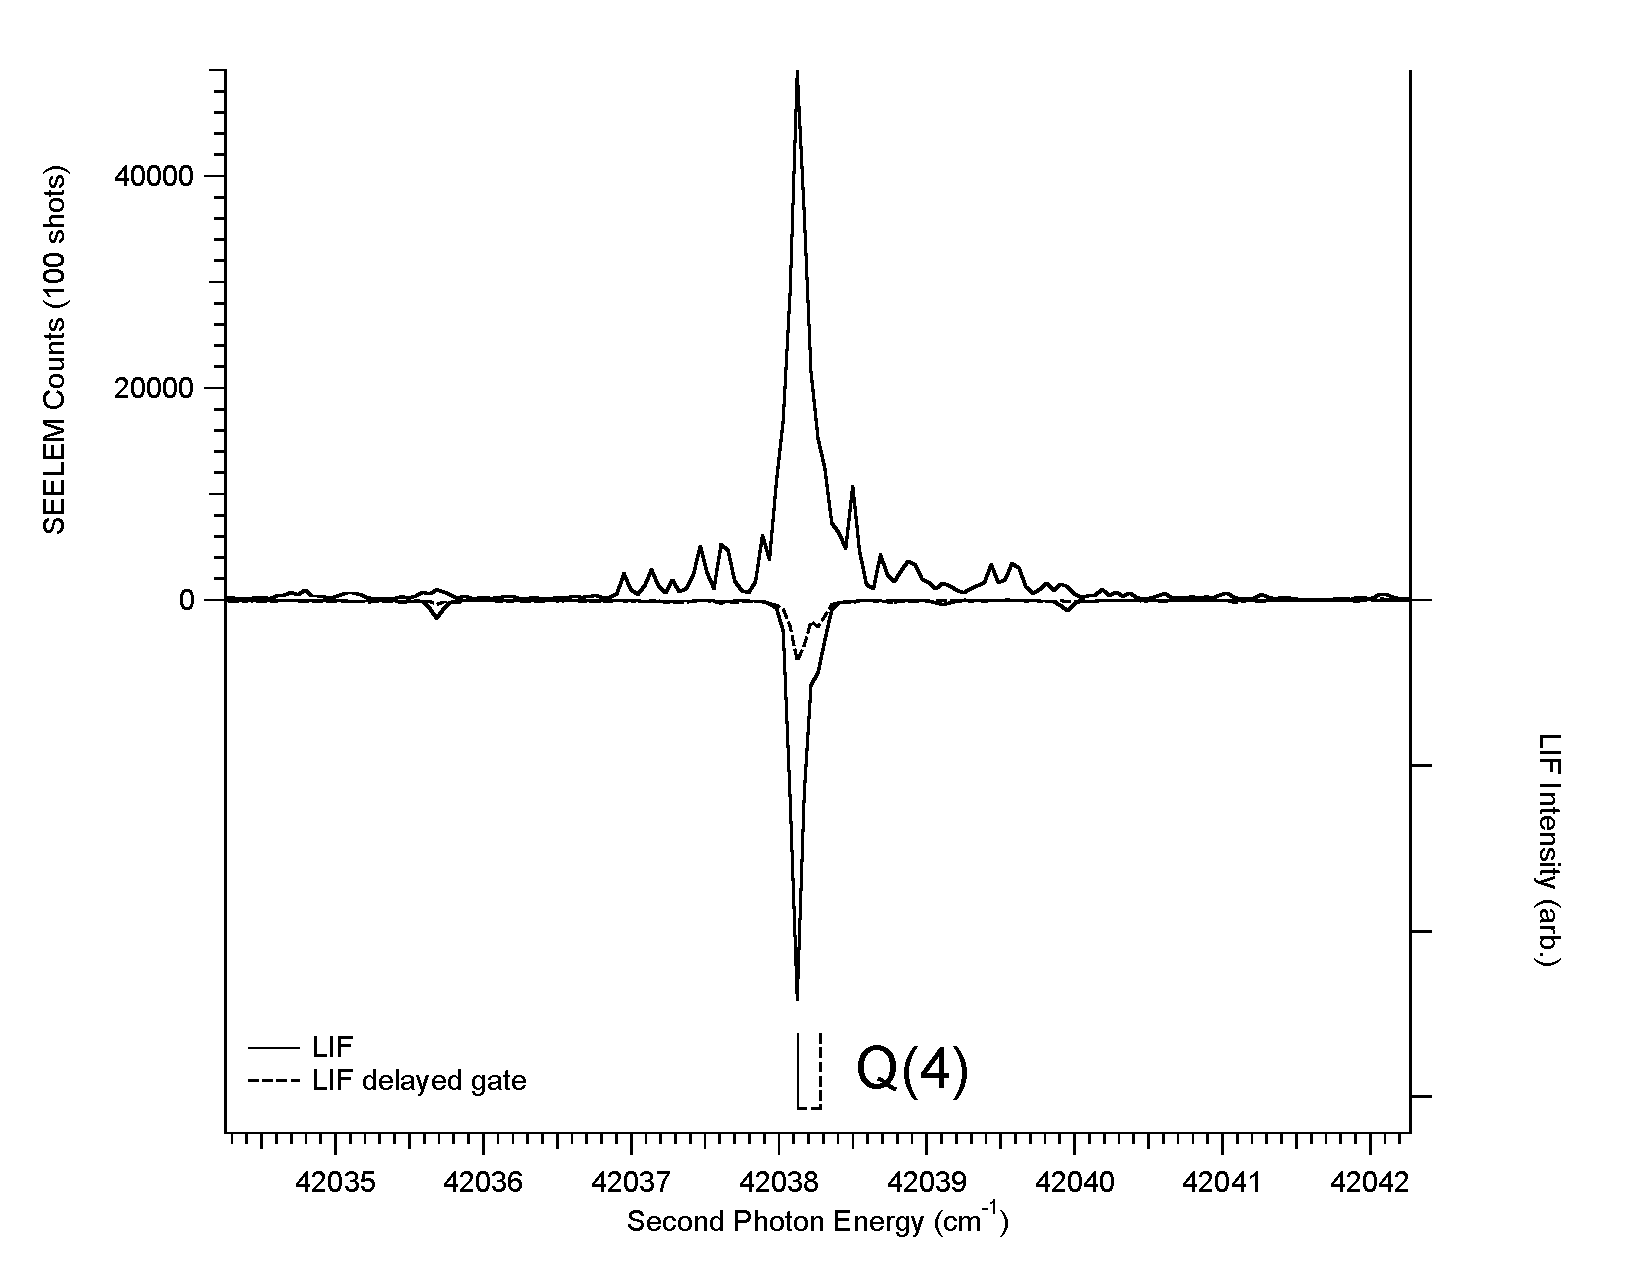
\includegraphics[width=6in]{spectrum-3361-q4-split.pdf}
  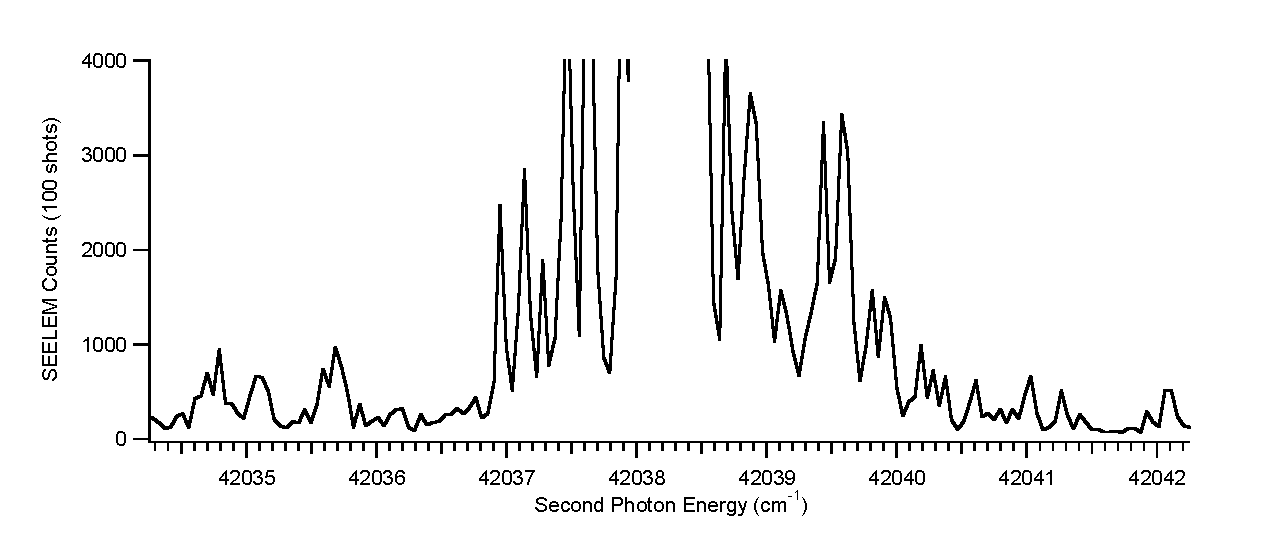
\includegraphics[width=6in]{spectrum-3361-q4-zoom.pdf}
\end{figure}

\begin{figure}
  \caption{Simultaneously recorded SEELEM (upper trace) and LIF (lower
    trace) spectra of the $3^36^1$ \Ka{0} sublevel of the \astate\
    state of \ce{C2H2}.  The R(4) line of the \xstate\ $\nu_3'' +
    \nu_4''$ level is used as an intermediate state in the experiment,
    so only the Q(5) line is observed in the upper state, according to
    Figure \ref{fig:levels-iruvdr}.  The LIF spectrum is integrated in
    two time regions: an early time window ($0.5\tau_s-2\tau_s$, solid
    trace) and a delayed time window ($10\tau_s-18\tau_s$, dashed
    trace).  No line splittings are observed in the LIF spectrum.}
  \label{fig:3361-q5}
  \centering
  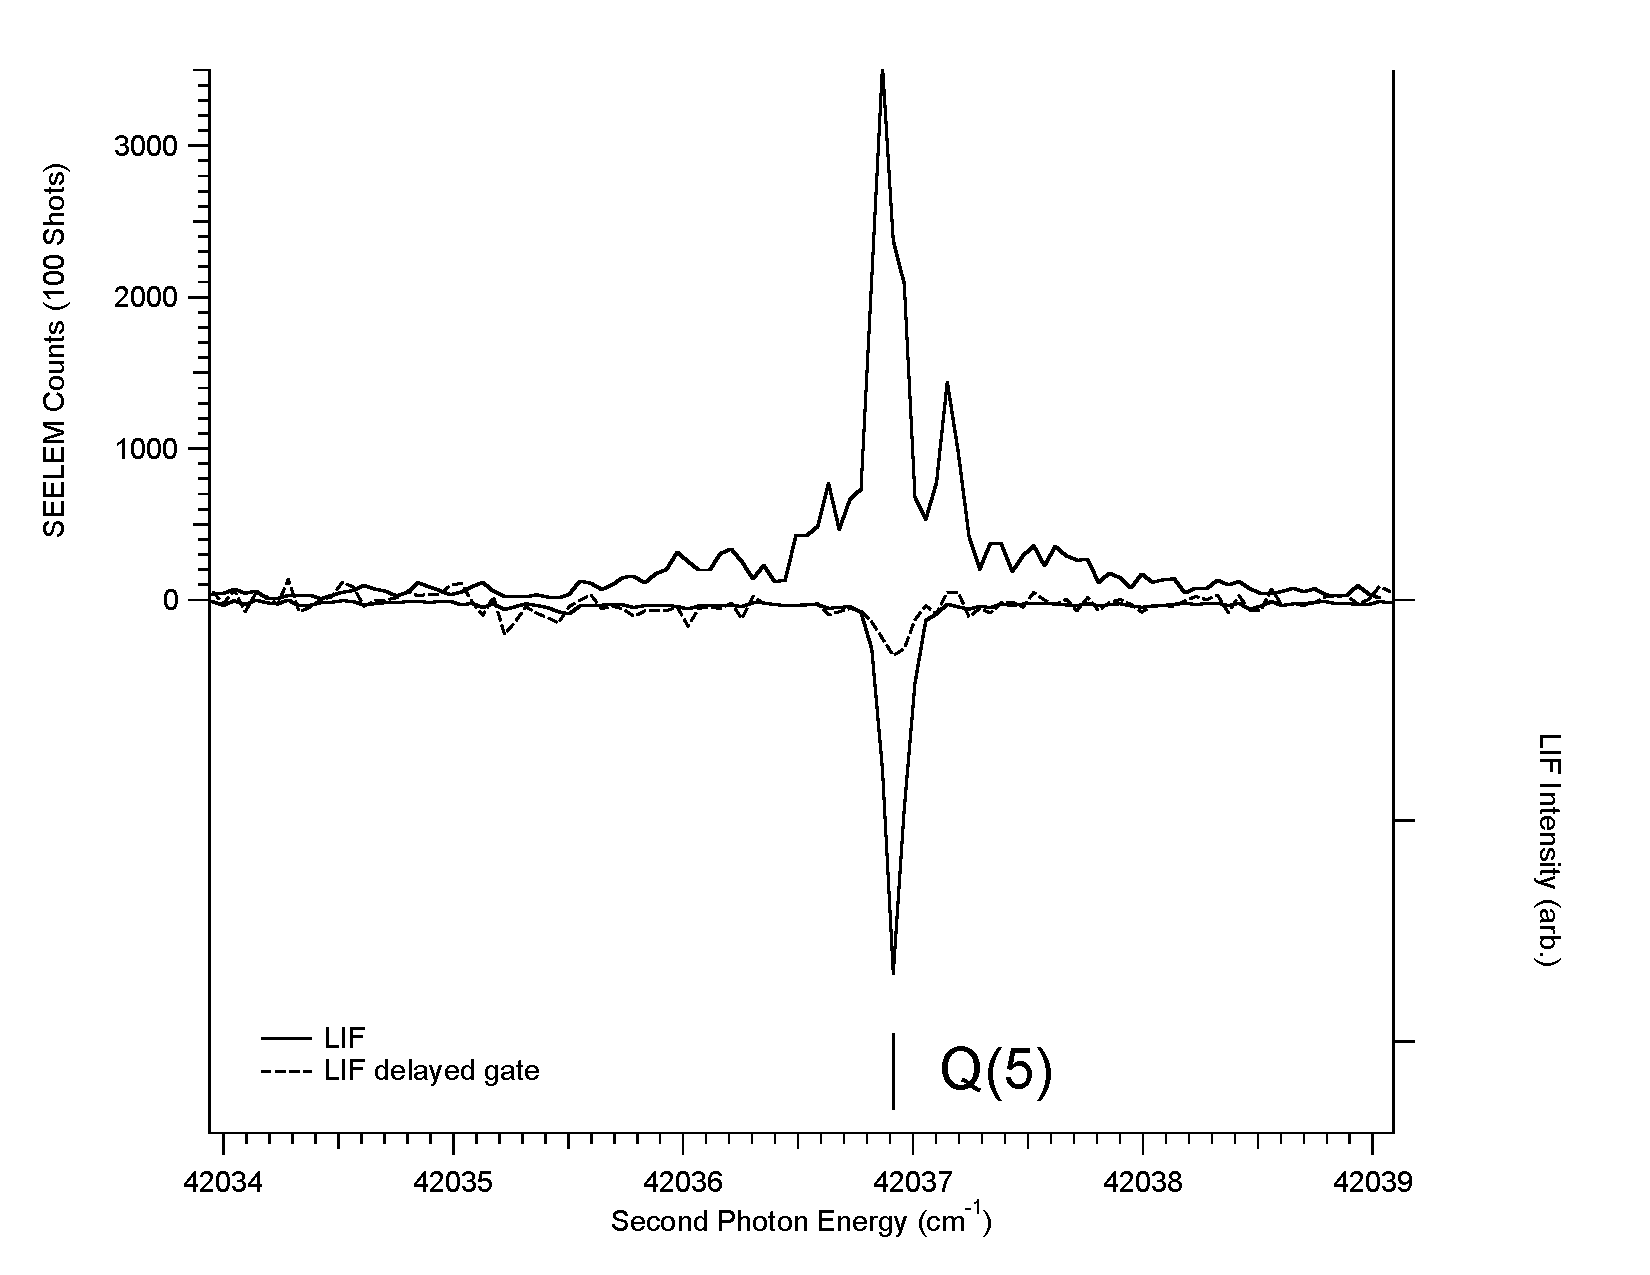
\includegraphics[width=6in]{spectrum-3361-q5-split.pdf}
  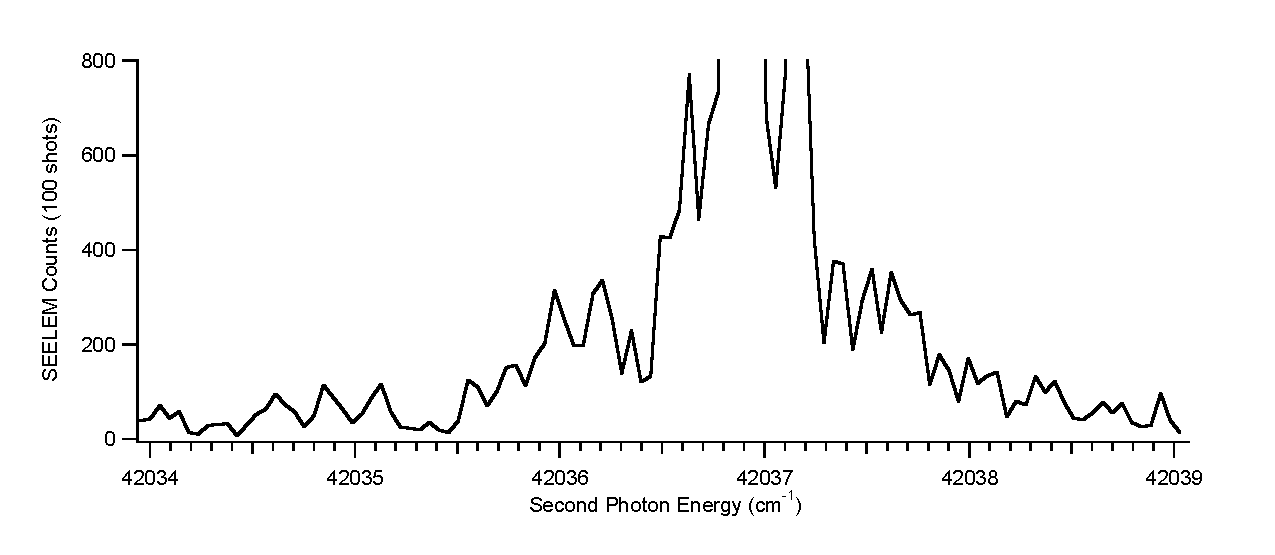
\includegraphics[width=6in]{spectrum-3361-q5-zoom.pdf}
\end{figure}

%%%%%%%%%%%%%%%%%%%%%%%%%%%%%%%%%%%%%%%%%%%%%%%%%%%%%%
%%
%% END OF 3^3 6^1 INDIV FIGURES
%%
%%%%%%%%%%%%%%%%%%%%%%%%%%%%%%%%%%%%%%%%%%%%%%%%%%%%%%

The spectrum of the $J'=0$ rotational level of $3^36^1$ \Ka{0} cannot
be recorded using the individual line double resonance method, since
the method permits only Q-branch transitions to appear in the UV
spectrum, and Q(0) transitions are strictly forbidden.  Instead, the
spectrum of $3^36^1$ \Ka{0} $J'=0$ was recorded in the region of the
P(1) transition by the survey method, using two relative polarization
geometries for the IR and UV laser beams.  Because selection rules for
$M_J$ make the P(1) transition forbidden in one geometry, a
``baseline'' spectrum can be recorded in the region of the P(1)
transition, and $J'=0$ levels can be distinguished from neighboring
$J'=1$ levels.  To evaluate the $M_J$ selection rules for the two-step
excitation, we choose to adopt a laboratory-fixed axis system where
the $z$-axis is the polarization axis of the IR laser, and the
$y$-axis is the direction of the colinear IR and UV laser propagation.
The reader is free to choose another laboratory-fixed axis system
under which to evaluate the selection rules.  The $M_J$ selection
rules are equally valid for all orientations of the laboratory-fixed
axes; our choice is determined by convenience and ease of explanation.

When the collinear IR and UV beams are perpedicularly polarized, the
P(1) transition, terminating on $J'=0$, is permitted in the UV.  The
IR excitation step proceeds according to the selection rule $\Delta
M_J=0$.  Magnetic sublevels in the intermediate state with $M_J=1$ are
populated from $M_J=1$ sublevels of the ground state.  In the second
excitation step, when the UV laser beam is perpedicularly polarized
relative to the IR beam, $\Delta M_J = \pm 1$ transitions are
permitted to the upper state $J'=0$ rotational level, which has only
one $M_J$ component, $M_J=0$.  Figure \ref{fig:levels-polarization}
illustrates the permitted transitions among $M_J$ sublevels as solid
arrows.

When the collinear IR and UV laser beams are polarized in parallel,
the selection rules for $\Delta M_J$ do not allow any transitions that
terminate in the upper state $J'=0$ rotational level.  Since the IR
and UV beams are both linearly polarized along the $z$-axis, $\Delta
M_J = 0$ in the IR and UV excitation steps.  The upper state has no
sublevels with $M_J=\pm 1$, so transitions beginning in the $M_J=\pm
1$ sublevels of the ground state may not proceed to the excited state.
A two-step excitation could possibly terminate in the $M_J=0$ level of
the excited state, if it were to start from $M_J=0$ in the ground
state.  However, such a transition is forbidden in the first step,
according to the selection rule that $M_J=0 \nleftrightarrow M_J=0$
for $\Delta J = 0$ (Q-branch) tansitions \cite{herzberg66}.  The
forbidden transition is illustrated with dashed arrows in Figure
\ref{fig:levels-polarization}.

%%%%%%%%%%%%%%%%%%%%%%%%%%%%%%%%%%%%%%%%%%%%%%%%%%%%%%%
%%
%% INSERT POLARIZATION DIAGRAM
%%
%%%%%%%%%%%%%%%%%%%%%%%%%%%%%%%%%%%%%%%%%%%%%%%%%%%%%%%

\begin{figure}
  \caption{Diagram of transitions among hyperfine levels terminating
    in the $J'=0$ rotational level of $3^36^1$ \Ka{0}.  When the IR
    and UV lasers are polarized in a perpendicular geometry,
    transitions terminating in the $J'=0$ rotational level of the
    excited state are permitted according to the selection rules
    $\Delta M_J = 0$ (first step), $\Delta M_J = \pm 1$ (second step).
    When the IR and UV lasers are polarized in a parallel geometry,
    transitions terminating in the $J'=0$ rotational level of the
    excited state are forbidden according to the selection rule $M_J =
    0 \nleftrightarrow M_J = 0$ when $\Delta J = 0$.}
  \label{fig:levels-polarization}

  \centering
  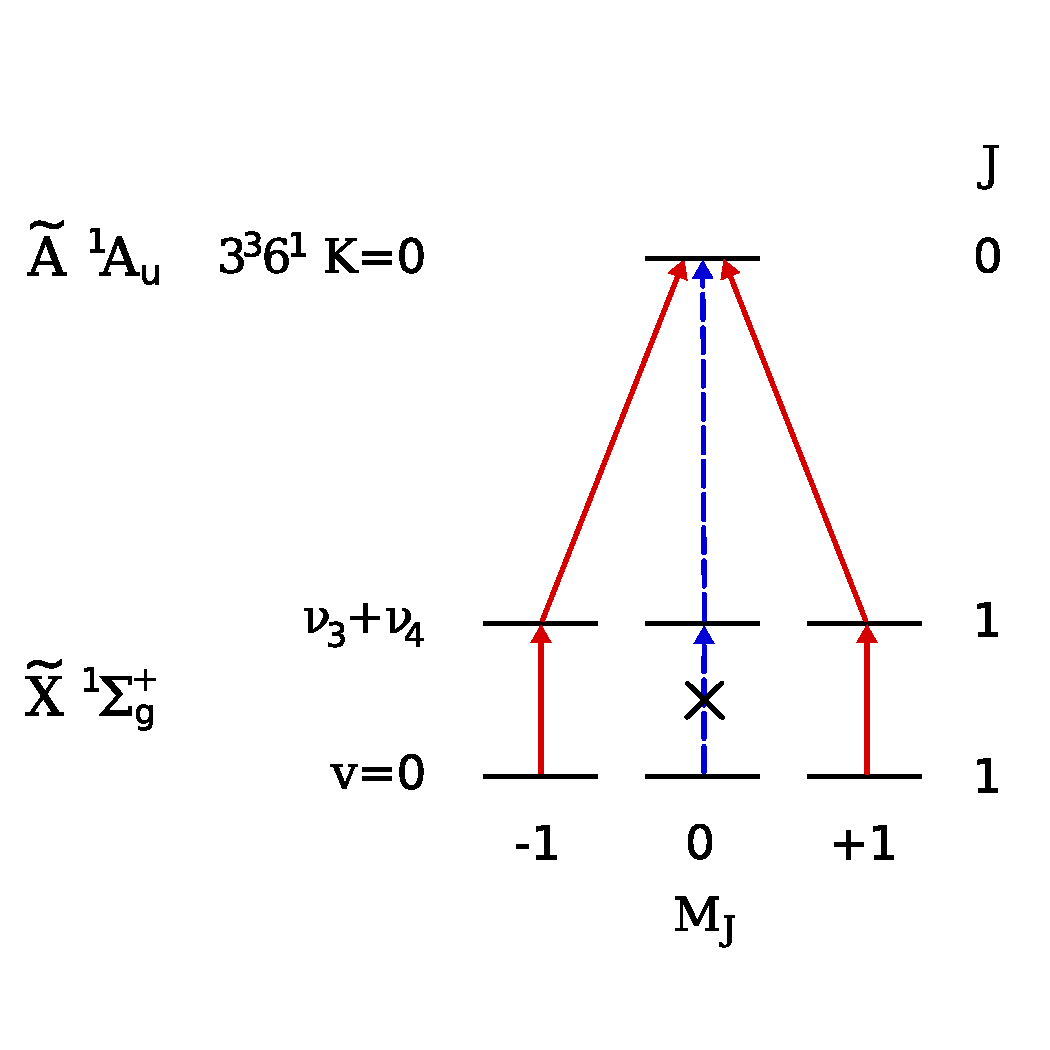
\includegraphics[width=5in]{levels-polarization.pdf}
\end{figure}

%%%%%%%%%%%%%%%%%%%%%%%%%%%%%%%%%%%%%%%%%%%%%%%%%%%%%%
%%
%% END POLARIZATION DIAGRAM
%%
%%%%%%%%%%%%%%%%%%%%%%%%%%%%%%%%%%%%%%%%%%%%%%%%%%%%%%

Simultaneously recorded SEELEM/LIF spectra in the region of the
$3^36^1$ \Ka{0} P(1) transition are shown in Figure
\ref{fig:3361-p1-polarization}, for perpendicular (solid trace) and
parallel (dashed trace) laser polarization.  Since the transition to
$J'=0$ is forbidden in the parallel geometry, the dashed trace serves
as a null spectrum in this region.  At UV frequencies between 42036.0
and 42041.3 \rcm, essentially all peaks in the SEELEM spectrum are due
to intensity borrowing from the $J'=0$ level of $3^36^1$ \Ka{0}.  This
particular region is shown with more detail in Figure
\ref{fig:3361-p1}.  The delayed LIF spectrum is also included as a
dashed trace in this figure.  A line splitting is resolved in the
delayed LIF spectrum, with the long-lifetime component lying to higher
frequency.

%%%%%%%%%%%%%%%%%%%%%%%%%%%%%%%%%%%%%%%%%%%%%%%%%%%%%%
%%
%% INSERT 3^3 6^1 POLARIZATION FIGURES HERE
%%
%%%%%%%%%%%%%%%%%%%%%%%%%%%%%%%%%%%%%%%%%%%%%%%%%%%%%%

\begin{figure}
  \caption{Simultaneously recorded SEELEM (upper trace) and LIF (lower
    trace) spectra of the $3^36^1$ \Ka{0} sublevel of the \astate\
    state of \ce{C2H2}.  The Q-branch of the \xstate\ $\nu_3'' +
    \nu_4''$ level is used as an intermediate transition in the
    experiment.  As a result, P- and R-branch lines are observed in
    the upper state, according to Figure \ref{fig:levels-iruvdr}.  The
    P(1) transition to the upper state is forbidden in a parallel
    IR-UV laser polarization geometry.  A spectrum recorded with this
    laser geometry is shown as a dashed line.  Lines appearing
    unambiguously in the SEELEM spectrum are indicated by solid
    arrows.  Lines indicated by dashed arrows are more uncertain.}
  \label{fig:3361-p1-polarization}
  \centering
  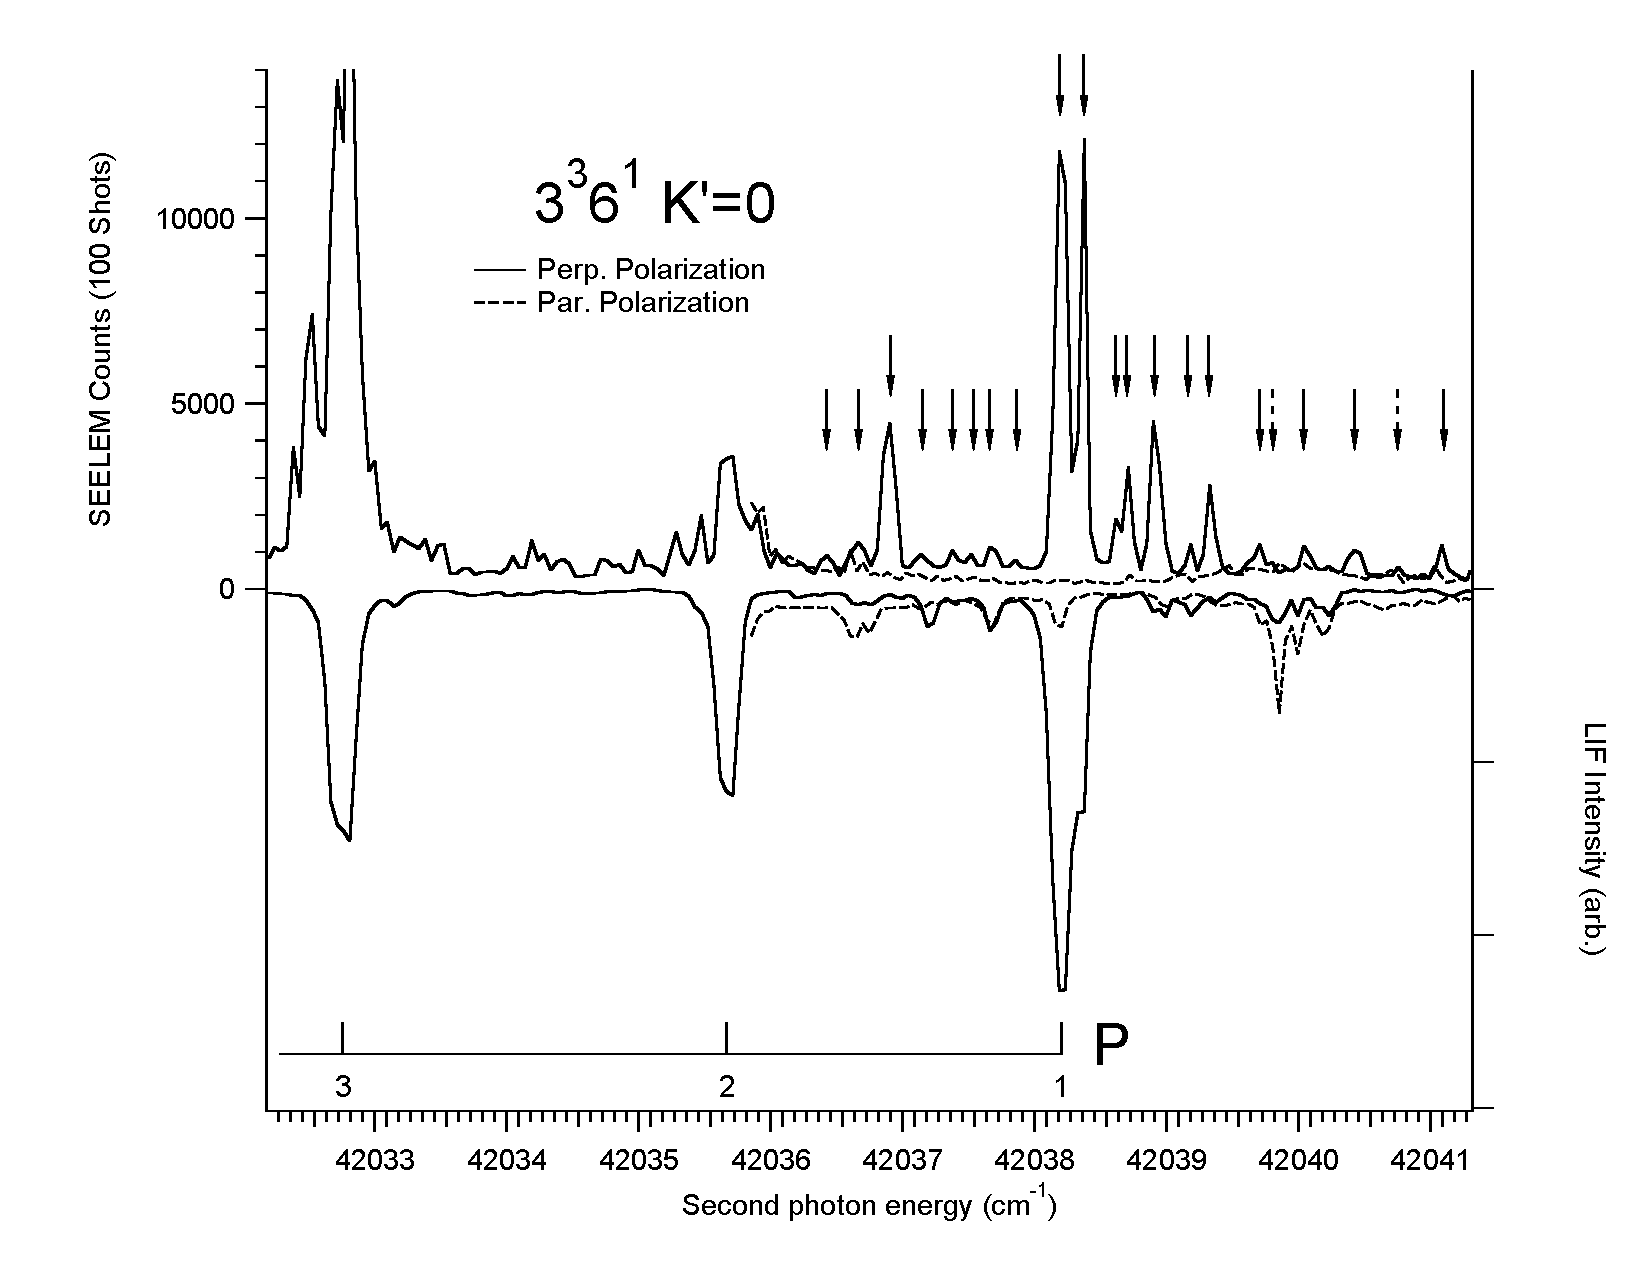
\includegraphics[width=7.3in,angle=90]{spectrum-3361-p1-polpeaks.pdf}
\end{figure}


\begin{figure}
  \caption{Simultaneously recorded SEELEM (upper trace) and LIF (lower
    trace) spectra of the $3^36^1$ \Ka{0} sublevel of the \astate\
    state of \ce{C2H2}.  The Q-branch of the \xstate\ $\nu_3'' +
    \nu_4''$ level is used as an intermediate transition in the
    experiment.  As a result, P- and R-branch lines are observed in
    the upper state, according to Figure \ref{fig:levels-iruvdr}.  The
    LIF spectrum is integrated in two time regions: an early time
    window ($0.5\tau_s-2\tau_s$, solid trace) and a delayed time
    window ($10\tau_s-18\tau_s$, dashed trace).  A line splitting of
    $\sim 2$ \rcm\ is observed in the LIF spectrum, with the
    longer-lifetime (nominally triplet) component located at higher
    energy.}
  \label{fig:3361-p1}
  \centering
  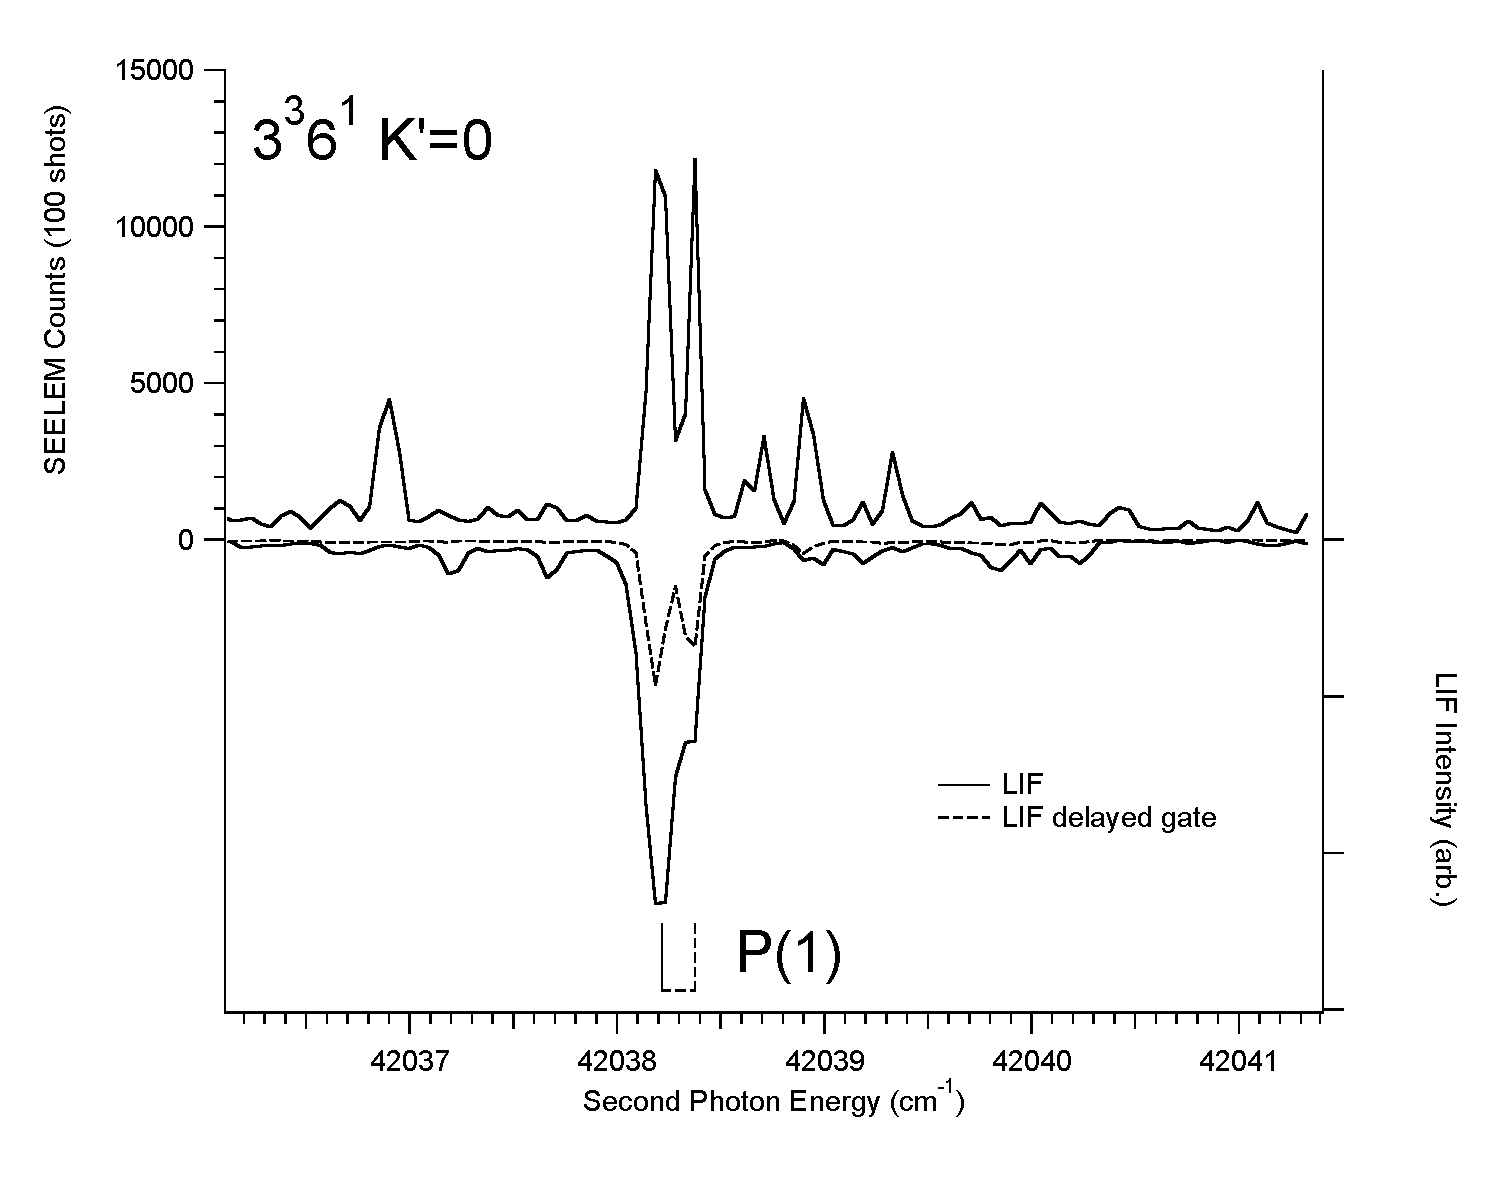
\includegraphics[width=5.8in]{spectrum-3361-p1-primed}
  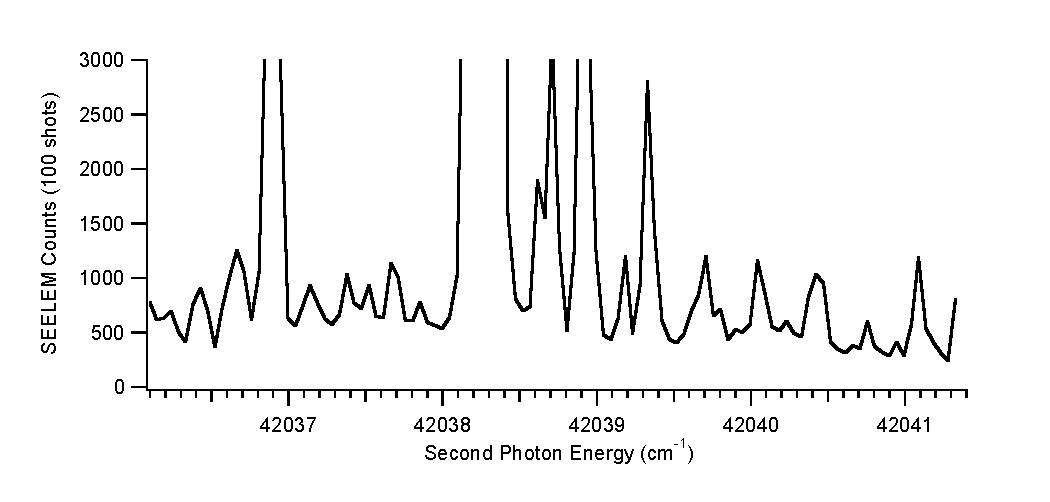
\includegraphics[width=6in]{spectrum-3361-p1-zoom}
\end{figure}

%%%%%%%%%%%%%%%%%%%%%%%%%%%%%%%%%%%%%%%%%%%%%%%%%%%%%%
%%
%% END OF 3^3 6^1 POLARIZATION FIGURES
%%
%%%%%%%%%%%%%%%%%%%%%%%%%%%%%%%%%%%%%%%%%%%%%%%%%%%%%%

The SEELEM/LIF spectrum of $3^34^1$ \Ka{0}, recorded by the survey
method, is shown in Figure \ref{fig:survey-3341}.  The LIF spectrum is
integrated in both early ($0.5\tau_s-2\tau_s$, solid trace) and
delayed ($10\tau_s-18\tau_s$, dashed trace) time windows.  Due to
saturation of the photomultiplier tube at early time intervals, the
early LIF spectrum shown in the figure was recorded and calibrated in
a separate scan.  The delayed LIF spectrum and the SEELEM spectrum
were acquired simultaneously.  The integrated SEELEM:LIF intensity
ratio is observed to be on the same order of magnitude as that of the
$3^36^1$ \Ka{0} level.

Line splittings appear in the delayed LIF spectrum of every transition
to the $3^34^1$ \Ka{0} sublevel.  The splittings span a frequency
range of $0.06-0.3$ \rcm.  The average frequency difference between
components of the same $J'$ is slightly larger than that of
$3^36^1$ \Ka{0}, and in general the splittings are more pronounced in the early
LIF spectrum.  Presumably the line splittings in $3^34^1$ \Ka{0} were
too small to be detected by Mizoguchi and coworkers, who recorded and
assigned the LIF spectrum of this level previously, and cite a UV
laser resolution of 0.1 \rcm \cite{mizoguchi00}.  Line splittings
reported in that reference, observed in another sublevel, are an order
of magnitude larger than those observed in this spectrum.

The line splitting in Q(1) could not be assigned directly from the
survey spectrum, because the long-lifetime component appears at a
frequency halfway between the Q(1) and Q(2) transitions.  To assign
the long-lifetime component, the spectrum of the P(2) transition in
$3^34^1$ \Ka{0} was recorded using the individual line method, via the
P(3) transition from the ground state.  This spectrum is shown in
Figure \ref{fig:3341-p2}.  A line splitting of -0.2 \rcm\ is observed
in the LIF spectrum, confirming the assignment of the long-lifetime
component in Q(1) (Figure \ref{fig:survey-3341}).

%%%%%%%%%%%%%%%%%%%%%%%%%%%%%%%%%%%%%%%%%%%%%%%%%%%%%%
%%
%% INSERT 3^3 4^1 FIGURES HERE
%%
%%%%%%%%%%%%%%%%%%%%%%%%%%%%%%%%%%%%%%%%%%%%%%%%%%%%%%

\begin{figure}
  \caption{Simultaneously recorded SEELEM (upper trace) and LIF (lower
    trace) spectra of the $3^34^1$ \Ka{0} sublevel of the \astate\
    state of \ce{C2H2}.  The Q-branch of the \xstate\ $\nu_3'' +
    \nu_4''$ level is used as an intermediate transition in the
    experiment.  As a result, Q-branch lines are observed in the upper
    state, according to Figure \ref{fig:levels-iruvdr}.  The LIF
    spectrum is integrated in two time regions: an early time window
    ($0.5\tau_s-2\tau_s$, solid trace) and a delayed time window
    ($10\tau_s-18\tau_s$, dashed trace).  Line splittings ranging from
    0.06 to 0.3 \rcm\ are observed in the delayed LIF spectrum of all
    rotational lines.  With one exception, the longer-lifetime
    (nominally triplet) components are located at lower energy than
    the shortest-lifetime (nominally singlet) component.}
  \label{fig:survey-3341}
  \centering
  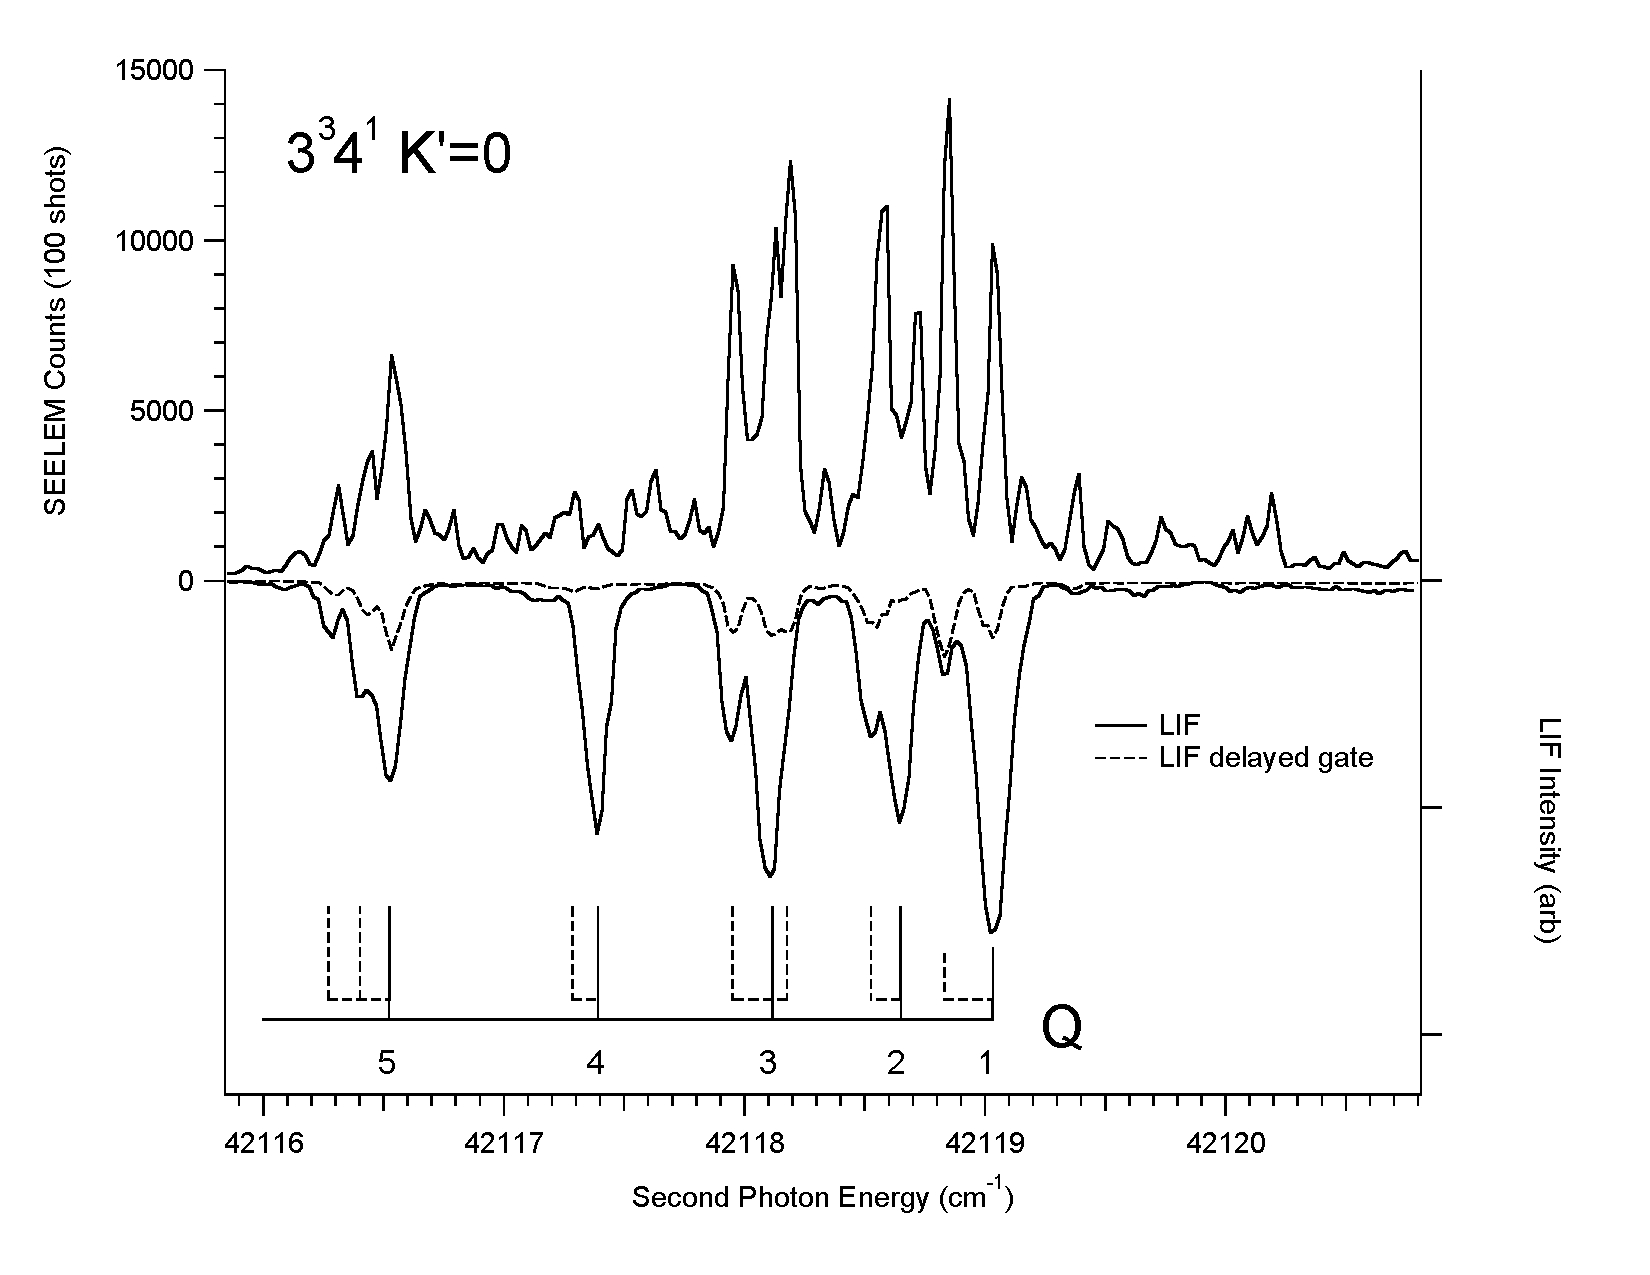
\includegraphics[width=7in,angle=90]{spectrum-3341-q5q1-primed.pdf}
\end{figure}

\begin{figure}
  \caption{Simultaneously recorded SEELEM (upper trace) and LIF (lower
    trace) spectra of the $3^34^1$ \Ka{0} sublevel of the \astate\
    state of \ce{C2H2}.  The P(3) line of the \xstate\ $\nu_3'' +
    \nu_4''$ level is used as an intermediate state in the experiment,
    so only the P(2) line is observed in the upper state, according to
    Figure \ref{fig:levels-iruvdr}.  The LIF spectrum is integrated in
    two time regions: an early time window ($0.5\tau_s-2\tau_s$, solid
    trace) and a delayed time window ($10\tau_s-18\tau_s$, dashed
    trace).  A line splitting of -0.2 \rcm\ is observed in the
    delayed fluorescence, confirming the assignment of the low-energy
    component as $J'=1$.}
  \label{fig:3341-p2}
  \centering
  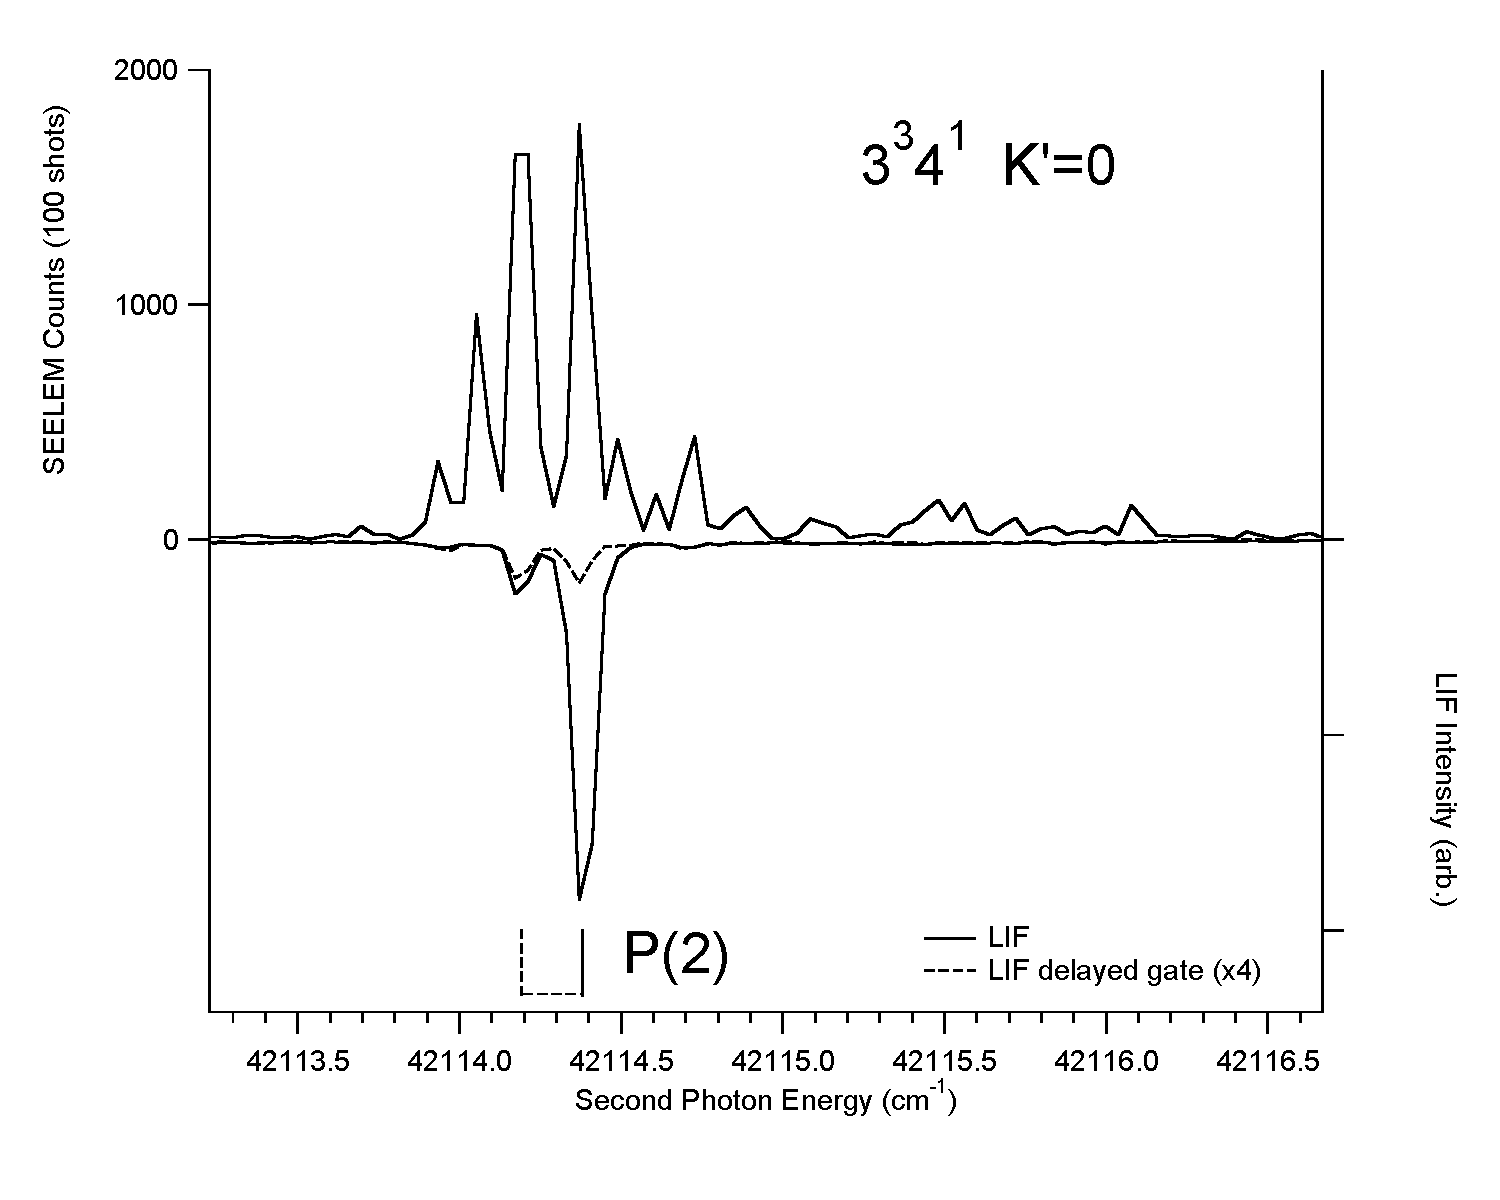
\includegraphics[width=6in]{spectrum-3341-p2-cal.pdf}
\end{figure}

%%%%%%%%%%%%%%%%%%%%%%%%%%%%%%%%%%%%%%%%%%%%%%%%%%%%%%
%%
%% END OF 3^3 4^1 FIGURES
%%
%%%%%%%%%%%%%%%%%%%%%%%%%%%%%%%%%%%%%%%%%%%%%%%%%%%%%%













































\section{Analysis}

\subsection{LIF Spectrum: \\Characterization of mediating $T_3$
  levels}

Line splittings on the order of $0.2$ \rcm\ were observed in the LIF
spectrum of both $S_1$ sublevels, $3^36^1$ \Ka{0} and $3^34^1$ \Ka{0}.
Because the extra lines appear with greater intensity in the delayed
LIF spectrum relative to the early LIF spectrum, they are attributed
to mixing between the $S_1$ sublevel and nearby triplet levels.  Three
triplet electronic states are energetically accessible: $T_1$, $T_2$,
and $T_3$.  According to the doorway model for acetylene, mixing
between $S_1$ levels and the manifold of $T_{1,2}$ triplet levels is
mediated by specific vibrational levels of the $T_3$ electronic state
\cite{dupre91, dupre95a, dupre95b, humphrey97, altunata00, mishra04}.
The average vibrational level spacing of $T_3$ is on the order of 10
\rcm, similar to that of $S_1$ \cite{thom07}.  In the majority of
cases, the $T_3$ levels, which mediate $S_1 \sim T_{1,2}$ mixing, do
not appear in the spectrum of an $S_1$ transition.  However, a
spectrum may still contain signatures of remote $T_3$ doorway
levels ($S_1 \sim T_3$ energy separation greater than 2 \rcm),
primarily as a result of the $J'$-dependence of $S_1 \sim T_3$ energy
denominators.  Four examples of this behavior are discussed in Chapter
4.

An analysis of the early vs. delayed LIF spectrum is our primary tool
for characterizing such distant doorway states.  In Chapter 4.3, it was
shown that a remote $T_3$ doorway level may give rise to a dependence of
the LIF center of gravity,
\begin{equation}
  E_{\text{ave}} = \int E \times I_t(E) \; dE,
\end{equation}
on time delay, $t$.  The effect results from drastically shorter
fluorescence lifetime for the nominal $S_1$ eigenstate relative to the
cluster of nearby, nominally triplet eigenstates.  The contrast in
fluorescence liftimes leads to changes in relative eigenstate
intensity as a function of time: at early times, the center of gravity
is dominated by the nominal $S_1$ state, while at longer delay times,
the center of gravity is dominated by nominally triplet eigenstates.
However, if the nominal $S_1$ eigenstate acquires more triplet
character, the contrast in fluorescence lifetimes is reduced,
deceasing the rate of change in center of gravity vs. time delay.

The relatively large line splittings observed in the spectrum of
$3^36^1$ \Ka{0} and $3^34^1$ \Ka{0} levels indicate that nominal $S_1$
eigenstates in these levels are appreciably singlet-triplet mixed.  To
make matters more complicated, the LIF spectra in this experiment
suffer from some saturation of the fluorescence signal at early time
delays, when the relative fluorescence intensity of the nominal $S_1$
state is at a maximum. We are thus precluded from using the center of
gravity vs. time as a diagnostic of the relative $T_3$ doorway energy,
as we were able to do with the spectrum of $3^3$ \Ka{2}, Chapter
4.5.4.

We rely, instead, on the positions and relative intensities of
resolved, long-lifetime lines as indicators of the relative $T_3$
doorway state energy.  In the spectrum of $3^34^1$ \Ka{0}, all
long-lived components are \emph{redshifted} from the energy of the
nominal $S_1$ state, with one exception.  The exception, occurring in
the Q(3) transition, warrants further examination.  The two observed
line splittings, indicated in Figure \ref{fig:survey-3341} by dashed
frequency markers, have frequencies of approximately $+0.1$ and $-0.2$
\rcm\ relative to the nominal $S_1$ state (solid frequency marker).
The intensities of both nominal triplet components are roughly
equivalent in the delayed LIF spectrum, indicating that the fractional
$S_1$ character of both states is approximately equal.

The ratio of fractional $S_1$ character may be used to estimate the
relative matrix elements for the two levels involved in the line
splitting.  Indirect mixing between $S_1$ and $T_{1,2}$ levels can be
evaluated by working in a mixed $S_1 \sim T_3$ basis, described in
Chapter 2.2.1.  In the mixed basis, the $S_1 \sim T_3$ spin-orbit
interaction is prediagonalized, resulting in a doorway-mixed $S_1$
state, $\ket{\tilde{s}}$, and an $S_1$-mixed doorway state,
$\ket{\tilde{\ell}}$.  Following Chapter 2, the ratio of $S_1$ and
$T_3$ amplitudes in $\ket{\tilde{s}}$ is determined by the mixing
angle $\alpha$ between the pure $S_1$ basis state, $\ket{s}$, and the
$T_3$ doorway, $\ket{\ell}$:
\begin{equation}
  \ket{\ts} = (1-\alpha^2)^{1/2} \ket{s} + \alpha \ket{\ell}.
\end{equation}
The basis states are defined such that $\alpha^2 \leq 0.5$.
The fractional $S_1$ character of a nominal $T_{1,2}$ eigenstate
$\ket{m}$ may be evaluated using perturbation theory:
\begin{equation}
  \label{eq:s-char}
  \begin{split}
    \lvert \braket{m|s} \rvert^2 
    &= \alpha^2 (1-\alpha^2) H_{\ell m}^2
    \left \lbrace 
      \frac{1}{\Delta E_{m \ts}} +
      \frac{1}{\Delta E_{m \tl}}
    \right \rbrace ^2\\
    &\approx \alpha^2 (1-\alpha^2) H_{\ell m}^2
    \frac{1}{\Delta E_{m \ts}^2}.
  \end{split}
\end{equation}
The approximate expression applies to remote doorway states, where the
energy separation $\Delta E_{m \ts}$ is much smaller than the energy
separation $\Delta E_{m \tl}$.  

Both triplet components observed in the vicinity of the Q(3)
transition interact with the same mixed-$S_1$ basis state, so the
$s,\ell$ mixing angle $\alpha$ is identical for both components, and
$\lvert \braket{m|s} \rvert^2 \propto H_{\ell m}^2 / \Delta E_{m
  \ts}^2$.  In Chapter 3 we showed that a doorway-mediated effective
Hamiltonian with one doorway state contains no interference pathways,
and as a result, the phases of all matrix elements may be taken to be
real and positive.  According to this property, the relative
magnitudes of the matrix elements $H_{\ell m}$ for two triplet levels
appearing in the delayed LIF spectrum of the same $S_1$ transition may
be determined using the expression
\begin{equation}
  \label{eq:approx-hlm}
  H_{\ell m} \propto \sqrt{ \Delta E_{m \ts}^2 \lvert \braket{m|s} \rvert^2 }
\end{equation}
For the Q(3) transition of $3^34^1$ \Ka{0}, the component appearing at
lower frequency must have approximately twice the matrix element with
the doorway state as the component appearing at higher frequency.

The pattern of line splittings is reversed in the delayed LIF spectrum
of $3^36^1$ \Ka{0}, shown in Figures
\ref{fig:3361-q1}$-$\ref{fig:3361-q5} and Figure \ref{fig:3361-p1}.
For this sublevel, all observed line splittings in the delayed LIF
spectrum are \emph{blueshifted} from the frequency of the nominal
$S_1$ state, with one exception.  This exception occurs in the Q(1)
transition, shown in Figure \ref{fig:3361-q1}.  Two additional lines
are observed in the delayed LIF spectrum, at frequencies of
approximately $+0.10$ and $-0.18$ \rcm, relative to the frequency of
the nominal $S_1$ eigenstate.  The ratio of line intensities is
approximately 2:1 in the delayed LIF spectrum, indicating that the
fractional $S_1$ character of the higher frequency state is
approximately twice as large as that of the lower frequency state.
The ratio of matrix elements $H_{\ell m}$ may be determined in the
same manner as before.  For this transition, the state appearing at
higher frequency must have a matrix element with the doorway state
approximately 0.78 times as large as that of the state appearing at
lower frequency.  With one exception just outlined, we find that the
long-lived states observed in the LIF spectrum of $3^36^1$ \Ka{0} are
blueshifted relative to the nominal $S_1$ state energy.

The $S_1 \sim T_3$ mixing angle, $\alpha$, is determined by the
matrix element and energy separation between the bright state and the
doorway state,
\begin{equation}
  \alpha = \frac{H_{s \ell}}{\Delta E_{s\ell}}.
\end{equation}
The matrix element, $H_{s \ell}$, can be estimated from the variance
of the LIF spectrum.  In Chapter 3, we showed that, for a
doorway-mediated Hamiltonian, the variance of the integrated LIF
spectrum,
\begin{equation}
  \label{eq:doorway-var}
  \sigma^2 = \int (E - E_s)^2 \times I(E) dE,
\end{equation}
is equal to the squared matrix element between the bright state and
the doorway state.  Consequently, the $S_1 \sim T_3$ matrix element
may be determined by taking the square root of the variance,
\begin{equation}
  H_{s \ell} = \sqrt{\sigma^2_{LIF}},
\end{equation}
under the condition that all LIF intensity supplied by the bright
state is observed in the spectrum.  When the doorway level is not
observed in the spectrum, this condition is not met, but the variance
of the LIF spectrum will certainly be smaller than the variance with
the doorway level included.  
%\TODO{Estimate total variance from
%  $\alpha, \Delta E$ when doorway is not observed.}  
Therefore, in the event that the doorway is not observed in the
spectrum, the variance of the LIF spectrum may be used as a lower
bound estimate for $H_{s \ell}^2$.

The approximate lower bound for the matrix element $H_{s \ell}$ was
determined from the variance of each LIF transition, calculated from
the integrated ($0.5\tau_s-18\tau_s$) LIF spectrum.  Our results are
summarized in Table \ref{table:lif-variances}.  The average lower
bound values of $H_{s \ell}$ for the $3^36^1$ \Ka{0} and $3^34^1$
\Ka{0} sublevels are on the order of 0.1 \rcm.  To make a comparison,
the matrix element for the local $T_3$ doorway level ($\Delta
E_{s\ell} < 0.3$ \rcm) observed in $S_1$ $3^3$ \Ka{1} was determined
to be approximately 0.1 \rcm\ \cite{mishra04}.  However, no local
doorway state is observed in the $3^36^1$ \Ka{0} and $3^34^1$ \Ka{0}
sublevels, so $\Delta E_{s\ell} > 2$ \rcm.  This indicates that the
$S_1 \sim T_3$ matrix elements for the $3^36^1$ \Ka{0} and $3^34^1$
\Ka{0} sublevels must be larger than that observed for the $3^3$
\Ka{1} sublevel.



\begin{table}
  \caption{Variance of the integrated LIF spectrum for each transition
    observed in the $S_1$ $3^34^1$ \Ka{0} and $3^36^1$ \Ka{0}
    sublevels.  The quantity $\sqrt{\sigma^2_{LIF}}$ is a lower bound
    for the $S_1 \sim T_3$ doorway matrix element, $H_{s\ell}$.  Also
    shown is the time-integrated center of gravity for each
    transition, $E_{ave}$, as well as the integration region used 
    in the analysis.}
  \label{table:lif-variances}
  \centering
  \vspace{5mm}
  \begin{tabular}{llll}
    & $E_{ave}$ & $\sqrt{\sigma^2_{LIF}}$ & Integration region \\
    \midrule
    \\
    $3^36^1$ \Ka{0} \\
    \\
    P(1) & 42038.24 & 0.097 & 42037.85$-$42038.60 \\
    Q(1) & 42040.35 & 0.118 & 42039.50$-$42041.00 \\
    Q(2) & 42039.84 & 0.089 & 42039.20$-$42040.50 \\
    Q(3) & 42039.14 & 0.085 & 42038.50$-$42039.50 \\
    Q(4) & 42038.15 & 0.083 & 42037.50$-$42038.80 \\
    Q(5) & 42036.93 & 0.095 & 42036.50$-$42037.50 \\
    \\
    $3^34^1$ \Ka{0} \\
    \\
    Q(1) & 42118.99 & 0.106 & 42118.76$-$42119.29 \\
    Q(2) & 42118.61 & 0.071 & 42118.36$-$42118.77 \\
    Q(3) & 42118.09 & 0.088 & 42117.74$-$42118.33 \\
    Q(4) & 42117.37 & 0.080 & 42117.00$-$42117.70 \\
    Q(5) & 42116.49 & 0.094 & 42116.13$-$42116.80 \\
  \end{tabular}
\end{table}

The observed patterns of splitting indicate that, if the local
singlet-triplet mixing is mediated by a non-local $T_3$ doorway, the
relative energy of the doorway is likely to be positive for the
$3^36^1$ \Ka{0} sublevel and negative for the $3^34^1$ \Ka{0}
sublevel.  This places both $T_3$ doorway states at a total energy
between 45937.8 \rcm\ and 46017.57 \rcm.  Since the $3^34^1$ \Ka{0}
and $3^36^1$ \Ka{0} sublevels are separated by about 80 \rcm\ in total
energy, it is unlikely that they mix primarily with the same doorway
state.  








%These follow a subset of the general rules for singlet$\sim$triplet
%transitions in polyatomic molecules originally discussed by Hougen
%\cite{hougen64}.  
% To be mixed by the spin orbit operator, two electronic states must
% differ in symmetry species by the species of rotation about the $a$,
% $b$, or $c$ axis \cite{stevens73}.  The $S_1$ and $T_3$ electronic
% states have $A$ and $B$ symmetry, respectively, and must be therefore
% connected by a rotation having $B$ symmetry.  Adopting a I$^r$
% convention in $C_2$ symmetry, we find that rotations about the $c$
% axis and the top axis ($a$) have the correct symmetry \cite{bunker98}.  
% % Show character tables and axis labels for \emph{trans}
% % acetylene.  Discuss the correspondence between the ($a,b,c$) axis
% % system and the ($x,y,z$).  See p.9, 18--19 in 4/2007--8/2007
% % notebook.

A brief discussion of selection rules for spin-orbit perturbations
lends some insight as to the possible identity of candidate $T_3$
doorway levels.  Selection rules for spin-orbit perturbations in
polyatomic molecules are given by Stevens and Brand, and have been
reformulated by other authors \cite{stevens73, howard78, dupre84}.
The total first-order spin-orbit matrix element between rovibrational
states of $S_1$ and $T_3$ is the product of three factors: an
electronic spin-orbit matrix element, a vibrational overlap factor,
and a rotational factor arising from angular momentum coupling.
Spin-orbit matrix elements follow the rotational selection rules
$\Delta J = 0$ and $\Delta P = 0$, where $P$ is the projection of $J$
on the top axis ($a$-axis) of the molecule \cite{hougen64}.  In Hund's
case ($b$), the quantum number $P$ is mixed among several levels with
different values of $K$, leading to the case ($b$) selection rule
$\Delta K = 0, \pm 1$ \cite{hougen64, stevens73}.

We express selection rules for spin-orbit perturbations in the
molecular symmetry group of the $T_3$ state, $C_2$, rather than the
symmetry group of $S_1$, $C_{2h}$.  The correspondence between the
$C_{2h}$ and $C_{2}$ symmetry groups can be made by simply removing
all $g$/$u$ labels from $C_{2h}$ operations.  One potential
complication arises, due to a possible reversal of the $b$ and $c$
inertial axes of a near-prolate top in $C_2$ symmetry.  However, the
vibration-rotation spin-orbit matrix elements are the same for both
cases, because the symmetry axis of twofold rotation remains
perpendicular to the inertial $a$-axis, regardless of the relative
orientation of the $b$ and $c$ axes \cite{hougen64}.

The three molecule-fixed spin functions, $\Gamma_{\sigma}$, transform
as rotations in the molecular symmetry group \cite{hougen64,
  stevens73}.  The symmetry of these functions,
$\Gamma_{\sigma}(J_a)$, $\Gamma_{\sigma}(J_b)$, and
$\Gamma_{\sigma}(J_c)$, determines the selection rules for $\Delta K$.
Mixing according to $\Delta K =0$ is permitted when the vibronic
symmetry of the $S_1$ and $T_3$ levels transforms as a rotation about
the top axis ($a$-axis), $^{ev}\Gamma_S \times ^{ev}\Gamma_T =
\Gamma_{\sigma}( J_a)$ \cite{stevens73}.  In the $C_2$ molecular
symmetry group, a rotation about the $a$-axis is of species $B$
\cite{bunker98}.

Taking into account the electronic symmetry of the $T_3$ state and the
vibronic symmetry of the $S_1$ $3^36^1$ and $3^34^1$ levels, the
vibrational symmetry of an admixed $T_3$ sublevel may be inferred.
Table \ref{table:delta-k} shows the relevant spin and vibronic
symmetries necessary to determine the $T_3$ vibrational symmetry. We
introduce the subscripted quantum numbers $K_T$ and $K_S$ to denote
the value of $K$ for the singlet ($S_1$) and triplet ($T_3$) vibronic
sublevels of interest.  A sublevel with $K_T=0$ must have a
vibrational symmetry of $b$ to mix with $S_1$ $3^36^1$ $K_S=0$.
Conversely, to mix with $S_1$ $3^34^1$ $K_S=0$, a $K_T=0$ sublevel
must have a vibrational symmetry of $a$.  Therefore, a $K_T=0$
sublevel may mix with either $3^36^1$ and $3^34^1$ $K_S=0$, but not
both.  Mixing according to $\Delta K =0$ is permitted when the
vibronic symmetry of the $S_1$ and $T_3$ levels transforms as a
rotation about the $b$ or $c$ axes, $^{ev}\Gamma_S \times
^{ev}\Gamma_T \supset \Gamma_{\sigma}(J_b)$ \emph{or} $\Gamma_{\sigma}(J_c)$
\cite{stevens73}.  Thus, a $K_T=1$ vibrational sublevel of any
symmetry may mix with a $K_S=0$ sublevel of any symmetry.

\begin{table}
  \caption{Spin-orbit perturbation selection rules between the $S_1$ $3^34^1$, 
    $3^36^1$ vibrational levels and vibrational levels of the $T_3$ 
    electronic state. Matrix elements for spin-orbit interaction may 
    be nonzero when the vibronic symmetry of the singlet and triplet 
    levels transforms as the appropriate molecule-fixed spin function,
    $\Gamma_{\sigma}$.  When $\Delta K = 0$, singlet sublevels may only 
    mix with $T_3$ sublevels of the same vibrational symmetry.  The 
    restriction is lifted when $\Delta K=1$.
  }
  \label{table:delta-k}
  \centering
  \begin{tabular}{llllrl}
    \\
    $S_1$ Level
    & $^{v}\Gamma_S$ & $^{ev}\Gamma_S$ & $\Gamma_\sigma$ & $\Delta K$ & $^{v}\Gamma_T$ \\
    \midrule
    
    $3^3 6^1$ 
    & $b$ & $^{1}B$ & $B$ & $0$ & $b$ \\
    & & & $A, B$ & $\pm1$ & $a, b$ \\
    
    $3^3 4^1$ 
    & $a$ & $^{1}A$ & $B$ & $0$ & $a$ \\
    & & & $A, B$ & $\pm1$ & $a, b$ \\[10pt]
    
  \end{tabular}\\[5mm]
  
  $C_{2}$ symmetry, $^{e}\Gamma_T =$ $^{3}B$
\end{table}

The rotational factors for spin-orbit matrix elements are
approximately independent of $J'$.  However, as discussed in Chapter
4, relative phases of rotational factors between two sublevels of the
same vibrational level may lead to interference effects.  Figure
\ref{fig:rotational-factors} shows the magnitudes and relative phases of
the rotational factors for spin-orbit matrix elements.  The energy
separation between $K_T=0$ and $K_T=1$ sublevels of the same $T_3$
vibrational level is on the order of 15$-$20 \rcm\ \cite{thom07}.  The total
spin-orbit matrix element between vibrational levels of $S_1$ and
$T_3$ may be as large as approximately 1 \rcm\ \cite{thom07}.  To mix
appreciably with both $K_T=0$ and $1$ sublevels of the same $T_3$
vibration, a sublevel of $S_1$ must have a total energy which is
midway between the triplet sublevels.

%%%%%%%%%%%%%%%%%%%%%%%%%%%%%%%%%%%%%%%%%%%%%%%%%%%%%%
%%
%% INSERT MATRIX ELEMENT FIGURE HERE
%%
%%%%%%%%%%%%%%%%%%%%%%%%%%%%%%%%%%%%%%%%%%%%%%%%%%%%%%

\begin{figure}
  \caption{Rotational factors of spin-orbit matrix elements between
    rovibrational levels of the $S_1$ and $T_3$ electronic states,
    where $K_S$=0.  A $K_S$=0 level may mix with $T_3$ levels with
    $K_T=0,1$.  Spin orbit perturbations are forbidden according to
    parity when $\Delta K = \Delta N = 0$.}
  \label{fig:rotational-factors}
  \centering
  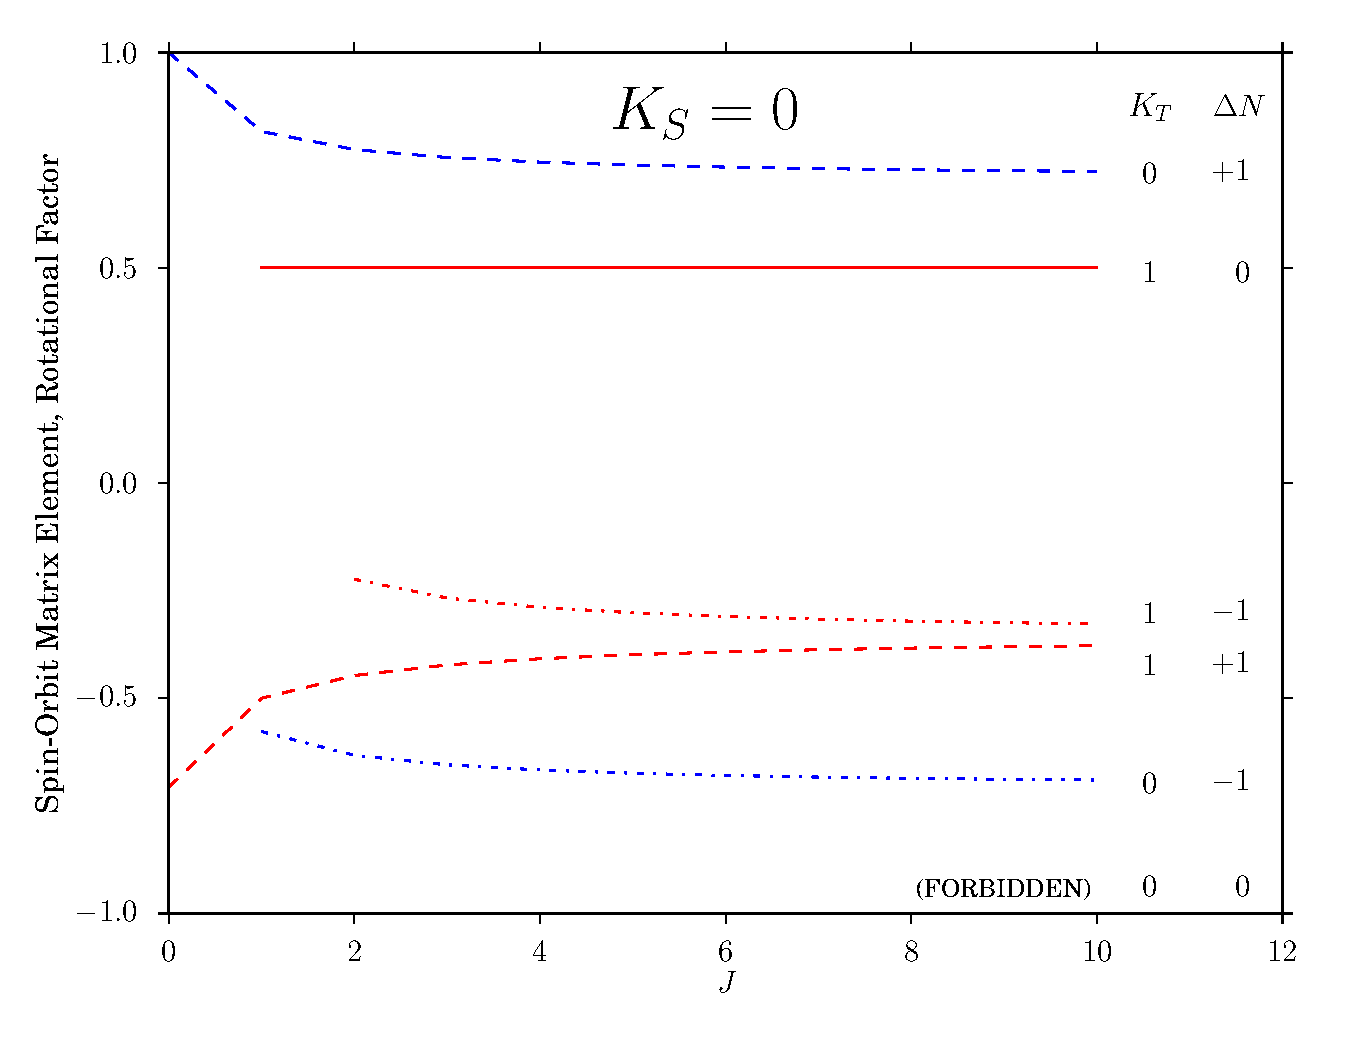
\includegraphics[width=6in]{rotational-factors-k0.pdf}
\end{figure}

%%%%%%%%%%%%%%%%%%%%%%%%%%%%%%%%%%%%%%%%%%%%%%%%%%%%%%
%%
%% END MATRIX ELEMENT FIGURE
%%
%%%%%%%%%%%%%%%%%%%%%%%%%%%%%%%%%%%%%%%%%%%%%%%%%%%%%%

The nonzero rotational factors for spin-orbit matrix elements are
illustrated on energy level diagrams in Figure \ref{fig:levels-k0} for
$K_T=0$ sublevels, and in Figure \ref{fig:levels-k1} for $K_T=1$
sublevels.  Figure \ref{fig:levels-k0} clearly illustrates that the
$3^36^1$ and $3^34^1$ $K_S=0$ sublevels may only mix with $K_T=0$
sublevels of the same vibrational symmetry.  Mixing with the $F_2$
component of a $K_T=0$ sublevel is forbidden, because the triplet
rotational level is of opposite parity.  Figure \ref{fig:levels-k1}
illustrates that triplet sublevels with $K_T=1$ contain levels of both
parities for each value of $J$ and $N$, therefore spin-rotation levels
of both parities are available for mixing with a $K_S=0$ singlet
rotational level.

%%%%%%%%%%%%%%%%%%%%%%%%%%%%%%%%%%%%%%%%%%%%%%%%%%%%%%
%%
%% INSERT SINGLET-TRIPLET FIGURES HERE
%%
%%%%%%%%%%%%%%%%%%%%%%%%%%%%%%%%%%%%%%%%%%%%%%%%%%%%%%


\begin{figure}
  \caption{Diagram of spin-orbit rotational selection rules between
    the $S_1$ $3^34^1$, $3^36^1$ \Ka{0} sublevels and $T_3$ sublevels
    with $K_T=0$.  When $K_T=K_S=0$, each singlet sublevel may only
    mix with zero-order triplet sublevels of the same vibrational
    symmetry.}
  \label{fig:levels-k0}
  \centering
  \vspace{5mm}
  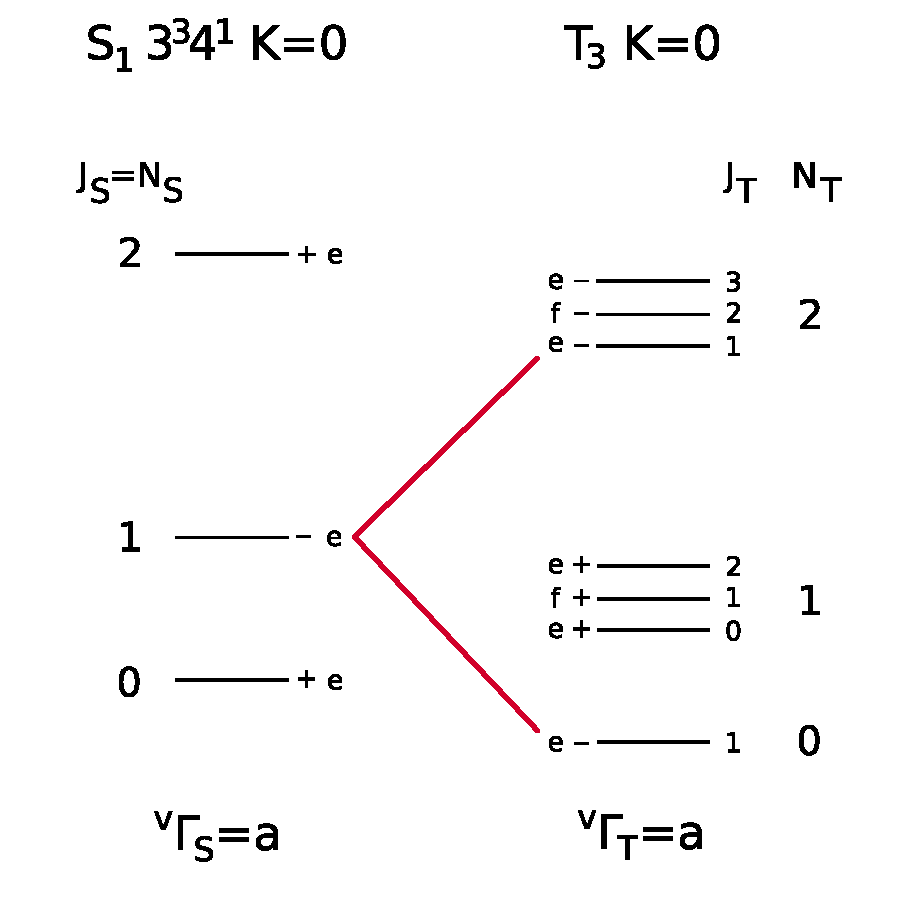
\includegraphics[width=4in,angle=90]{levels-3341}
  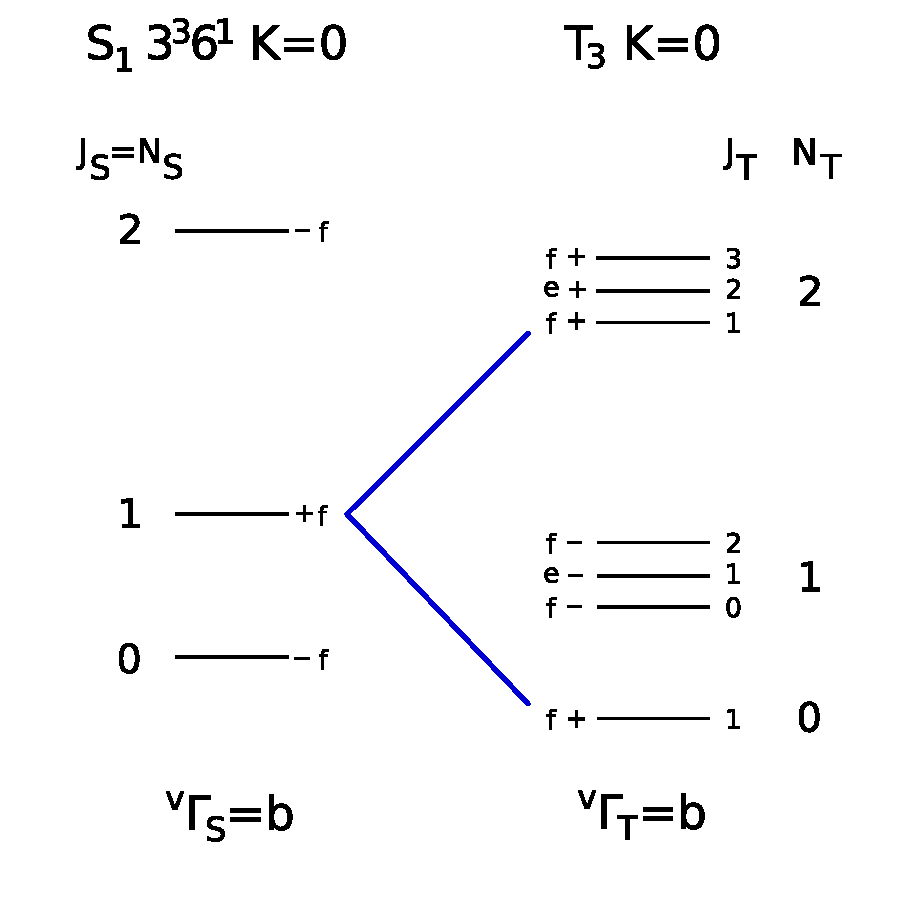
\includegraphics[width=4in,angle=90]{levels-3361}  
\end{figure}

\begin{figure}
  \caption{Diagram of spin-orbit rotational selection rules between
    the $S_1$ $3^34^1$, $3^36^1$ \Ka{0} sublevels and $T_3$ sublevels
    with $K_T=1$.  In this case, mixing is not restricted by
    vibrational symmetry, and the singlet sublevels are permitted to
    mix with the same zero-order triplet sublevel.}
  \label{fig:levels-k1}
  \centering
  \vspace{5mm}
  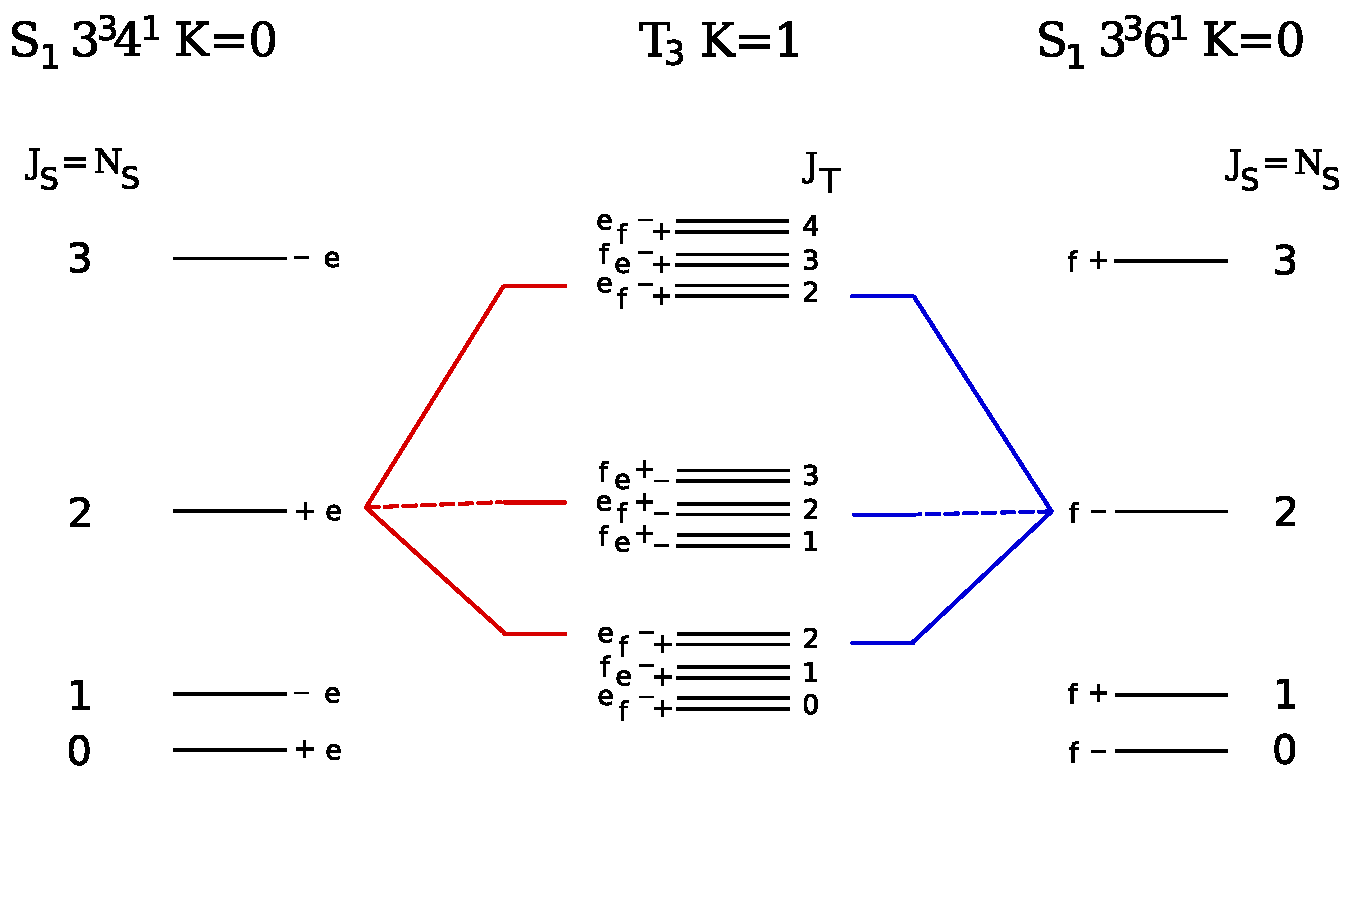
\includegraphics[width=6in,angle=90]{levels-k1}
\end{figure}

%%%%%%%%%%%%%%%%%%%%%%%%%%%%%%%%%%%%%%%%%%%%%%%%%%%%%%
%%
%% END SINGLET-TRIPLET FIGURES
%%
%%%%%%%%%%%%%%%%%%%%%%%%%%%%%%%%%%%%%%%%%%%%%%%%%%%%%%

Having surveyed the vibronic symmetry restrictions and rotational
selection rules for spin-orbit perturbations, we investigate the
propensities of vibrational overlap integrals between vibrational
levels of $S_1$ and $T_3$.  Harmonic frequencies for the $T_3$
electronic surface have been reported by Bryan Wong, who carried out a
high-level \emph{ab initio} calculation of the $S_1$ and $T_3$
electronic surfaces \cite{wong07}.  A significant challenge in this
work was the diabatization of the $T_2$ and $T_3$ electronic surfaces
along two strongly coupled modes, the antisymmetric CH stretch and the
\emph{cis}-bend \cite{thom07}.  The vibrational modes of $S_1$ and
$T_3$ are numbered differently, since the equilibrium geometry of the
$T_3$ electronic state has $C_2$ symmetry.  The vibrations of both
electronic states are identified in Table \ref{table:vibration-ids}.
The frequency of the $T_3$ torsional vibration, $\nu_2$, is twice as
large as the corresponding $S_1$ vibration, $\nu_4$.  Conversely, the
frequencies of the $T_3$ \emph{trans} and \emph{cis}-bending
vibrations, $\nu_4$ and $\nu_6$, are significantly smaller than those
in $S_1$.

\begin{table}
  \caption{The vibrational normal modes of the $S_1$ and $T_3$
    electronic states. The
    position of the torsional mode is changed in $T_3$ relative to
    $S_1$, because $g/u$ symmetry operations are not present in the 
    $C_2$ molecular symmetry group of $T_3$.
  }
  \label{table:vibration-ids}
  \centering
  \vspace{5mm}
  \begin{tabular}{llc}
    \toprule
    $S_1$\\
    $\nu_1$ ($a_g$) & symmetric CH stretch \\
    $\nu_2$ ($a_g$) & CC stretch \\
    $\nu_3$ ($a_g$) & \emph{trans}-bend \\
    $\nu_4$ ($a_u$) & torsion \\
    $\nu_5$ ($b_u$) & antisymmetric CH stretch \\
    $\nu_6$ ($b_u$) & \emph{cis}-bend \\
    \\
    $T_3$\\
    $\nu_1$ ($a$) & symmetric CH stretch \\
    $\nu_2$ ($a$) & torsion \\
    $\nu_3$ ($a$) & CC stretch \\
    $\nu_4$ ($a$) & \emph{trans}-bend \\
    $\nu_5$ ($b$) & antisymmetric CH stretch \\
    $\nu_6$ ($b$) & \emph{cis}-bend \\
    \bottomrule
  \end{tabular}
\end{table}

Using the results of this \emph{ab initio} calculation, Thom and
coworkers reported vibrational overlap integrals between $S_1 \:\;
3\nu_3$ and nearby levels of $T_3$ \cite{thom07}.  The harmonic
approximation of Sharp and Rosenstock was used to calculate the
overlap integrals, which is accuate enough to give a general idea of
the relative energy and magnitude of the vibrational overlap
\cite{sharp64}.  Using the programs published by Bryan Wong in his
thesis, we have carried out an identical calculation for the $S_1$
$3\nu_3+\nu_4$ and $3\nu_3+\nu_6$ levels \cite{wong07}.  Our results
are summarized in Tables \ref{table:overlap-4} and
\ref{table:overlap-6}.

For both $S_1$ levels, we find at least one vibrational level of $T_3$
within 300 \rcm\ that has an extremely large ($\sim 0.1$) overlap
integral.  When levels with the largest absolute overlap integrals
are considered, we observe that the $T_3$ \emph{trans}-bending
vibration ($\nu_4$) and torsional vibration ($\nu_2$) are observed to
promote vibrational overlap with $S_1$ $3\nu_3+\nu_4$.  For $S_1$
$3\nu_3+\nu_6$, the $T_3$ levels with the five largest absolute
vibrational overlap integrals contain quanta in both the \emph{trans}
and \emph{cis}-bending vibrations ($\nu_4$ and $\nu_6$).



\begin{table}
  \caption{Calculated vibrational overlap integrals between $S_1 \:\; 
    3\nu_3+\nu_4$ and levels of $T_3$ within an energy separation of 
    300 \rcm.  The energies and vibrational overlap integrals are 
    calculated in the harmonic approximation, according to the methods
    outlined by Thom and coworkers \cite{thom07}.  Integrals with an 
    absolute magnitude of less than $1\times 10^{-6}$ are not shown, 
    including those that are zero by symmetry.  The five vibrational levels 
    of $T_3$ with the largest absolute vibrational overlap integrals 
    are marked with a ($\triangleright$).  One $T_3$ level, 
    containing 6 quanta of the \emph{trans}-bending vibration ($\nu_4$), 
    is calculated to have an extremely large vibrational overlap integral 
    ($\sim$ 0.1) with $S_1 \:\; 3\nu_3+\nu_4$.  Overall, the $T_3$ 
    \emph{trans}-bending vibration and torsional vibration ($\nu_2$) are 
    observed to promote vibrational overlap.  The mean and median of the 
    absolute values of the $T_3$ vibrational overlap integrals for $S_1 \:\; 
    3\nu_3+\nu_4$ are shown below the table.}
  \label{table:overlap-4}
\centering
\vspace{5mm}
  \begin{tabular}{llcc}
\toprule
& $T_3$ vibrational level & $E - E(S_1 \:\; 3\nu_3+\nu_4)$ (\rcm) & Overlap integral \\
\midrule
                 & $\nu_1 + \nu_4$                               &  -294 &  0.0022 \\
$\triangleright$ & $ 2 \nu_2 + \nu_4$                            &  -267 &  0.037 \\
$\triangleright$ & $ 6 \nu_4$                                    &  -255 &  0.12 \\
                 & $10 \nu_6$                                    &  -198 & -0.0002 \\
                 & $\nu_2 +  6 \nu_6$                            &  -161 & -0.0002 \\
                 & $\nu_1 +  2 \nu_6$                            &  -152 &  0.0002 \\
                 & $\nu_3 +  4 \nu_4$                            &  -149 & -0.027 \\
                 & $ 2 \nu_2 +  2 \nu_6$                         &  -124 &  0.0032 \\
                 & $ 5 \nu_4 +  2 \nu_6$                         &  -113 &  0.011 \\
                 & $\nu_4 + \nu_5 + \nu_6$                       &   -86 & -0.014 \\
                 & $ 2 \nu_3 +  2 \nu_4$                         &   -43 & -0.025 \\
                 & $\nu_3 +  3 \nu_4 +  2 \nu_6$                 &    -7 &  0.0081 \\
$\triangleright$ & $ 4 \nu_4 +  4 \nu_6$                         &    29 & -0.028 \\
                 & $\nu_5 +  3 \nu_6$                            &    56 & -0.0021 \\
                 & $ 3 \nu_3$                                    &    62 & -0.0013 \\
$\triangleright$ & $\nu_2 +  4 \nu_4$                            &    66 &  0.080 \\
                 & $ 2 \nu_3 + \nu_4 +  2 \nu_6$                 &    99 & -0.0047 \\
                 & $\nu_3 +  2 \nu_4 +  4 \nu_6$                 &   135 & -0.0025 \\
                 & $ 3 \nu_4 +  6 \nu_6$                         &   171 &  0.0059 \\
$\triangleright$ & $\nu_2 + \nu_3 +  2 \nu_4$                    &   172 &  0.056 \\
                 & $\nu_2 +  3 \nu_4 +  2 \nu_6$                 &   208 & -0.023 \\
                 & $ 2 \nu_3 +  4 \nu_6$                         &   241 & -0.0004 \\
                 & $\nu_3 + \nu_4 +  6 \nu_6$                    &   277 & -0.0004 \\
                 & $\nu_2 +  2 \nu_3$                            &   277 &  0.0047 \\
\midrule
& & Mean overlap integral (abs. val.): & 0.019 \\
& & Median overlap integral (abs. val.): & 0.0053 \\
  \end{tabular}\\[3mm]

\end{table}

\begin{table}
  \caption{Calculated vibrational overlap integrals between $S_1 \:\; 
    3\nu_3+\nu_6$ and levels of $T_3$ within an energy separation of 
    300 \rcm.  The energies and vibrational overlap integrals are 
    calculated in the harmonic approximation, according to the methods
    outlined by Thom and coworkers \cite{thom07}.  Integrals with an 
    absolute magnitude of less than $1\times 10^{-6}$ are not shown, 
    including those that are zero by symmetry.  The five vibrational levels 
    of $T_3$ with the largest absolute vibrational overlap integrals 
    are marked with a ($\triangleright$).  One $T_3$ level, 
    containing 3 quanta of the \emph{trans}-bending vibration ($\nu_4$) 
    and one quantum of the \emph{cis}-bending vibration ($\nu_6$), is 
    calculated to have an extremely large vibrational overlap integral 
    ($\sim$ 0.2) with $S_1 \:\; 3\nu_3+\nu_6$.  All five $T_3$ levels
    with the largest absolute vibrational overlap factors contain a combination
    of the $T_3$ \emph{trans} and \emph{cis}-bending vibrations
    ($\nu_4$ and $\nu_6$).  The mean and median of the absolute values 
    of the vibrational overlap integrals for $S_1 \:\; 3\nu_3+\nu_6$ 
    are larger than those for $S_1 \:\; 3\nu_3+\nu_4$ by less than a 
    factor of two.
  }
  \label{table:overlap-6}
  \centering
  \vspace{6mm}
  \begin{tabular}{llcc}
\toprule
& $T_3$ vibrational level & $E - E(S_1 \:\; 3\nu_3+\nu_6)$ (\rcm) & Overlap integral \\
\midrule
$\triangleright$ & $\nu_2 +  3 \nu_4 + \nu_6$                    &  -281 & -0.21 \\
                 & $ 2 \nu_3 +  3 \nu_6$                         &  -248 &  0.0007 \\
                 & $\nu_3 + \nu_4 +  5 \nu_6$                    &  -212 &  0.0085 \\
                 & $ 2 \nu_4 +  7 \nu_6$                         &  -175 &  0.010 \\
                 & $\nu_2 + \nu_3 + \nu_4 + \nu_6$               &  -175 & -0.040 \\
                 & $\nu_2 +  2 \nu_4 +  3 \nu_6$                 &  -139 & -0.039 \\
                 & $\nu_3 +  7 \nu_6$                            &   -69 &  0.0007 \\
                 & $\nu_4 +  9 \nu_6$                            &   -33 &  0.0039 \\
                 & $\nu_2 + \nu_3 +  3 \nu_6$                    &   -33 & -0.0025 \\
                 & $\nu_2 + \nu_4 +  5 \nu_6$                    &     3 & -0.017 \\
                 & $\nu_1 + \nu_4 + \nu_6$                       &    12 & -0.0039 \\
$\triangleright$ & $ 2 \nu_2 + \nu_4 + \nu_6$                    &    40 &  0.057 \\
$\triangleright$ & $ 6 \nu_4 + \nu_6$                            &    52 & -0.084 \\
                 & $ 2 \nu_4 + \nu_5$                            &    78 & -0.027 \\
                 & $11 \nu_6$                                    &   109 &  0.0005 \\
                 & $\nu_2 +  7 \nu_6$                            &   146 & -0.0015 \\
                 & $\nu_1 +  3 \nu_6$                            &   154 & -0.0006 \\
$\triangleright$ & $\nu_3 +  4 \nu_4 + \nu_6$                    &   157 &  0.090 \\
                 & $ 2 \nu_2 +  3 \nu_6$                         &   182 &  0.0040 \\
                 & $\nu_3 + \nu_5$                               &   184 & -0.0018 \\
                 & $ 5 \nu_4 +  3 \nu_6$                         &   194 &  0.0095 \\
                 & $\nu_4 + \nu_5 +  2 \nu_6$                    &   220 &  0.0085 \\
                 & $ 2 \nu_3 +  2 \nu_4 + \nu_6$                 &   263 & -0.0061 \\
$\triangleright$ & $\nu_3 +  3 \nu_4 +  3 \nu_6$                 &   299 & -0.051 \\
\midrule
& & Mean overlap integral (abs. val.): & 0.028 \\
& & Median overlap integral (abs. val.): & 0.0085 \\
  \end{tabular}\\[3mm]
\end{table}



Although specific $T_3$ doorway levels cannot be identified from our
spectra, the relative energy of $T_3$ doorways is determined from line
splittings that appear in the delayed LIF spectra of $S_1$ $3^36^1$
\Ka{0} and $3^34^1$ \Ka{0}.  The magnitudes of the spin-orbit matrix
element between the $S_1$ level and the doorway level are estimated
from the variance of the LIF spectrum.  Additionally, the allowed
vibrational symmetries of $T_3$ doorway states are discussed above in
terms of spin-orbit selection rules for $\Delta K$.  To investigate
the possible identity of $T_3$ doorway levels, we use the previously
reported programs of Bryan Wong to calculate vibrational overlap
integrals.  The vibrational overlap integral calculations indicate
that the $T_3$ \emph{trans}-bending vibration ($\nu_4$) and torsional
vibration ($\nu_2$) have a propensity to increase vibrational overlap
with $S_1 \:\; 3\nu_3 + \nu_4$, while a combination of the $T_3$
\emph{trans} and \emph{cis}-bending ($\nu_6$) vibrations is observed
to increase vibrational overlap with $S_1 \:\; 3\nu_3 + \nu_6$.





















% Use Bryan's program to compute overlap integrals for the two bands.

% Show number of modes available in each symmetry as a function
% of energy.



\subsection{SEELEM Spectrum: \\Characterization of the local manifold of
  $T_{1,2}$ levels}

The SEELEM spectrum shows the distribution of nominal $T_{1,2}$
eigenstates that have approximately 0.25\% fractional $S_1$ character.
This specificity in SEELEM detection probability, discussed in Chapter
4.3.1, arises from the competing effects of excitation probability,
electron ejection probability and survival probability.  When the
$T_3$ doorway level is energetically distant ($\Delta E > 1$ \rcm),
the envelope of SEELEM-detectable states is not expected to exhibit
large interference effects, as observed in $S_1$ $3^3$ \Ka{1}.
Interference effects in the SEELEM spectrum result from a cross term
in the equation for SEELEM detection probability, described in Chapter
2.3.3.

Levels of the $T_1$ and $T_2$ electronic states are observed to be
extensively mixed in this energy region, evidenced by the widely
varying Land\'{e} $g$-factors observed in Zeeman Anticrossing (ZAC)
spectra \cite{dupre95a}.  (Although many of the states observed in the
ZAC experiments are nominally $S_0$, the authors rule out extensive
$S_0 \sim T_{1,2}$ mixing as the underlying cause for the widely
varying $g$-factors.  Such mixing would cause the average $g$-factor
to be approximately zero as discussed in Section 5.1 of
\cite{dupre95a}.)

We adopt a simple model, based on the classic work of Bixon and
Jortner, to address $T_3 \sim T_{1,2}$ mixing \cite{bixon68}.  Mixing
between a bright state and an ensemble of equally spaced dark states
with identical matrix elements results in a Lorentzian distribution of
fractional bright state character, $a^2$.  The full width at half
maximum of the distribution is
\begin{equation}
  \label{eq:bixon-model}
  \Gamma = 2 \pi v^2 \rho_m,
\end{equation}
where $v$ is the bright$\sim$dark matrix element (held constant in the
model), and $\rho_m$ is the density of dark states.  Since the $S_1$
level is only indirectly coupled to the manifold of $T_{1,2}$ levels,
the parameter $v$ in equation \ref{eq:bixon-model} must be related to
the matrix elements of a doorway-mediated effective Hamiltonian.  In
equation \ref{eq:s-char}, it can be seen that the effective squared
matrix element between a $T_{1,2}$ level and the $S_1$ level is
$\alpha^2 (1 - \alpha^2) H_{\ell m}^2$.  When $\alpha < 0.25$, the
product $\alpha^2 (1 - \alpha^2) \approx \alpha^2$.  The Lorentzian
parameter $v$ is thus related to the doorway-mediated Hamiltonian
model as $v^2 \approx \alpha^2 H_{\ell m}^2$.

Another challenge is that the SEELEM signal is not proportional to
fractional bright state character.  The SEELEM detection probability
is a function of fractional $S_1$ and $T_3$ character, and includes
factors for laser excitation, survival probability, and electron
ejection probability \cite{humphrey97}.  In Chapter 2, we showed that
if the doorway state is remote ($\Delta E_{s\ell} > 2$ \rcm), the
fractional $T_3$ character follows an approximate proportionality to
the fractional $S_1$ character.  Under these circumstances, the SEELEM
intensity equation simplifies to
\begin{equation}
  \label{eq:simple-lem}
  P_{\text{SEELEM}} \propto a^4 \times \exp(-R \; a^2),
\end{equation}
where $R$ is the ratio of the SEELEM detector flight time (309
\microsec) to the fluorescence lifetime of the $S_1$ electronic state
(270 ns), approximately equal to 1144 in this study.  The polynomial
factor is the product of laser excitation and electron ejection
probabilities, and the exponential factor represents the probability
that a molecule will not fluoresce before arriving at the SEELEM
detector surface.  The combination of the two factors results in a
maximum of SEELEM detection probability when the fractional $S_1$
character is approximately $2/R_m \approx 0.0017$, less than one
percent.  

On the outer edge of the SEELEM intensity distribution, we assume that
the fractional $S_1$ character of the SEELEM-detectable eigenstates
approaches zero.  In this limit, the SEELEM detection probability is
dominated by the polynomial factor, and is proportional to the
fractional bright state character squared.  Surprisingly, this causes
a \emph{narrowing} effect on the outer edge of the SEELEM intensity
distribution, relative to the Lorentzian distribution of fractional
bright state character.  The fundamental cause of this effect is the
sampling of a non-time-integrated intensity.  Because the SEELEM
detector samples the population of metastable molecules only at a
particular time, the normalization conditions for conservation of
fractional bright state character result in a squared Lorentzian
distribution.  The full width of a squared Lorentzian distribution is
approximately 0.64 times the full width of a standard Lorentzian.

Such an argument may seem to conflict with Kevin Cunningham's
measurements of SEELEM lifetimes in acetylene as relatively uniform
and universally less than 280 \microsec\ \cite{cunningham-thesis}.
However, an upper limit on fluorescence lifetime of 280 \microsec\
means that the survival probability is approximately constant for all
SEELEM-detectable states.  It follows that the SEELEM detection
probability depends primarily on the product of laser exitation and
electron ejection factors, leading to a Lorentzian-type distribution
of intensity in the SEELEM spectrum.

The SEELEM spectra recorded with the individual line method were fit to
Lorentzian envelopes.  To carry out the fit, the SEELEM spectrum was
first smoothed to approximately twice the average level spacing, using
a Hamming window function for convolution.  A Lorentzian profile was
fit to the smoothed spectrum using a non-linear least-squares
regression.  Figure \ref{fig:seelem-fits} shows the best-fit
Lorentzian profiles obtained for the $J'=1-5$ rotational levels of
$3^36^1$ \Ka{0}.  The Lorentzian FWHM, $\Gamma$, varies between 0.39 and
0.59 \rcm.  From these values, the product $v^2 \rho_m$ is determined
to be approximately $\Gamma / (2 \pi) \approx 0.078$ \rcm.  

The density of states is determined by direct count.  The simple
formula
\begin{equation}
\rho_m = \frac{n}{\Delta E}
\end{equation}
was used, where $n$ is the number of lines in the SEELEM spectrum, and
$\Delta E$ is the energy difference between the lowest and highest
energy line.  Lines in the SEELEM spectrum were identified simply by
finding local maxima.  State densities for the spectra in Figure
\ref{fig:seelem-fits} are listed in Table \ref{table:seelem-params}.
It is likely that a direct count underestimates the number of nominal
$T_{1,2}$ eigenstates, since the incoherent laser linewidth is only a
factor of three less than the average line spacing.  Drabbels and
co-workers reported density of states measurements for the $3^3$
\Ka{1} sublevel using a high-resolution (18 MHz) laser
\cite{drabbels94}.  Their estimates, spanning a smaller frequency
range, exceed our observation by 1 to 4 times.

\begin{table}
  \caption{Estimation of the product $\alpha H_{\ell m}$ from the
    SEELEM spectra of five transitions in $S_1$ $3^36^1$ \Ka{0}.  The
    quantity $\alpha$ represents the $S_1 \sim T_3$ mixing angle in a
    single doorway-mediated effective Hamiltonian, and the $H_{\ell
      m}$ represents the doorway $\sim T_{1,2}$ matrix element (held 
    constant) in a simple statistical coupling model. The fitted
    Lorentzian width for the SEELEM spectrum, $\Gamma_{SEELEM}$, and 
    the directly-counted density of $T_{1,2}$ states, $\rho_m$, are
    used to determine $\alpha H_{\ell m}$.}
  \label{table:seelem-params}
  
  \centering
  \vspace{5mm}
  \begin{tabular}{llll}
    \toprule
    Transition & $\Gamma_{\text{SEELEM}}$ (\rcm) & $\rho_m$ (states /
    \rcm) & $\alpha H_{\ell m}$ (\rcm)\\
    \midrule
    Q(1) & 0.387 & 5.66 & 0.104 \\
    Q(2) & 0.558 & 5.66 & 0.125 \\
    Q(3) & 0.585 & 6.24 & 0.122 \\
    Q(4) & 0.391 & 5.66 & 0.105 \\
    Q(5) & 0.506 & 5.93 & 0.116 \\
    \midrule
    & 0.49(8) & 5.8(2) & 0.114(8)\\
    \end{tabular}
\end{table}

From the density of states measurement, we may estimate the parameter
$v^2 \approx (0.0134$ \rcm$)^2$.  Following the relation $v^2 \approx
\alpha^2 H_{\ell m}^2$, we estimate the product $\alpha H_{\ell m}$ as
$0.116$ \rcm.  The final formula for this important molecular
porperty, according to the simple model, is
\begin{equation}
  \alpha H_{\ell m} = \sqrt{\frac{\Gamma}{f \; 2 \pi \; \rho_m}},
\end{equation}
where $f$ is a factor describing the change in the width of the
intensity distribution resulting from a non-time-integrated
measurement, described above.  According to this formula, a possible
underestimation of the state density would cause the estimate of
$\alpha H_{\ell m}$ to be higher than the true value.  Potential
narrowing effects caused by the sampling a non-time-integrated
spectrum would cause the estimate of $\alpha H_{\ell m}$ to be
slightly lower than its true value.  Our estimates of $\alpha H_{\ell
  m}$ are shown in Table \ref{table:seelem-params}, for the five
transitions in $3^36^1$ \Ka{1} recorded via the individual line
method.

% The full width at half maximum (FWHM) of the SEELEM distribution is
% derived in Chapter 2, in terms of the $S_1 \sim T_3$ mixing angle,
% $\alpha$, and the average $T_3 \sim T_{1,2}$ matrix element,
% $H_{T_3T_{1,2}}$.  Our results led to the following formula:
% \begin{equation}
%   \text{FWHM} = 
%     \frac{2}{\sqrt{e R_m}} 
%     \left \lvert 
%       \alpha \: H_{H_{T_3T_{1,2}}}
%     \right \rvert, 
% \end{equation}
% where $R_m$ is a constant equal to the zero-order $S_1$ fluorescence
% lifetime divided by the flight time to the SEELEM detector.  The
% zero-order $S_1$ fluorescence lifetime of acetylene \astate\ is
% approximately 270 ns \cite{ochi91}.  The molecular flight time from
% the point of excitation to the SEELEM surface was measured as 309
% \microsec\ in this study.  Evaluating this equation using the average
% observed SEELEM full width at half maximum, 0.49 \rcm, we arrive at a
% value of approximately 30 \rcm\ for the product $\alpha \times
% H_{H_{T_3T_{1,2}}}$.


%%%%%%%%%%%%%%%%%%%%%%%%%%%%%%%%%%%%%%%%%%%%%%%%%%%%%%
%%
%% INSERT SEELEM FIT FIGURES
%%
%%%%%%%%%%%%%%%%%%%%%%%%%%%%%%%%%%%%%%%%%%%%%%%%%%%%%%

\begin{figure}
  \caption{Lorentzian fitting results for the $J'=1-5$ SEELEM spectra
    of the $3^36^1$ \Ka{0} sublevel.  The parameter $\Gamma$, equal to
    the half-width of the distribution, is proportional to the product
    of the $S_1 \sim T_3$ mixing angle and the average $T_3 \sim T_{1,2}$
    matrix element.  The value of $\Gamma$ is given in units of \rcm.}
  \label{fig:seelem-fits}
  \vspace{5mm}
  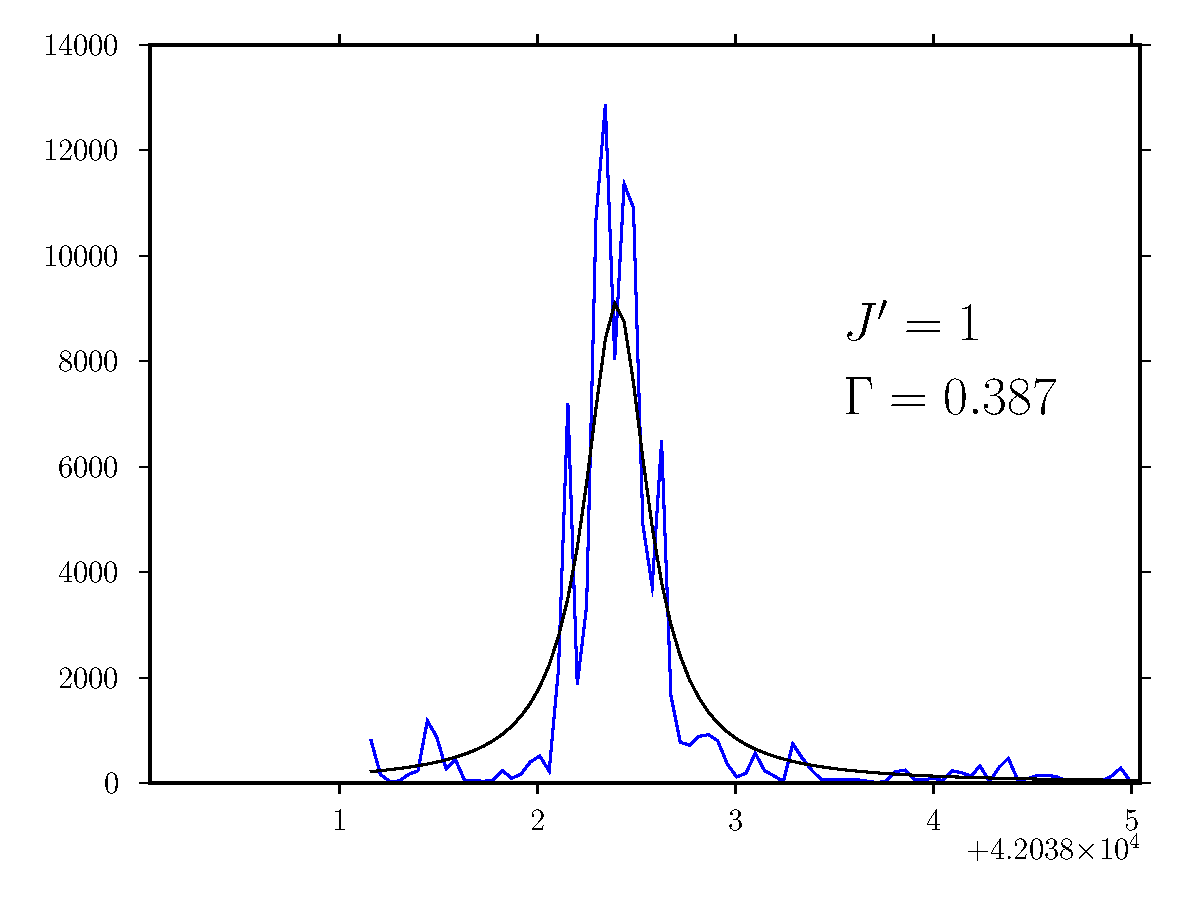
\includegraphics[width=3.2in]{3361-q1-seelemfit}
  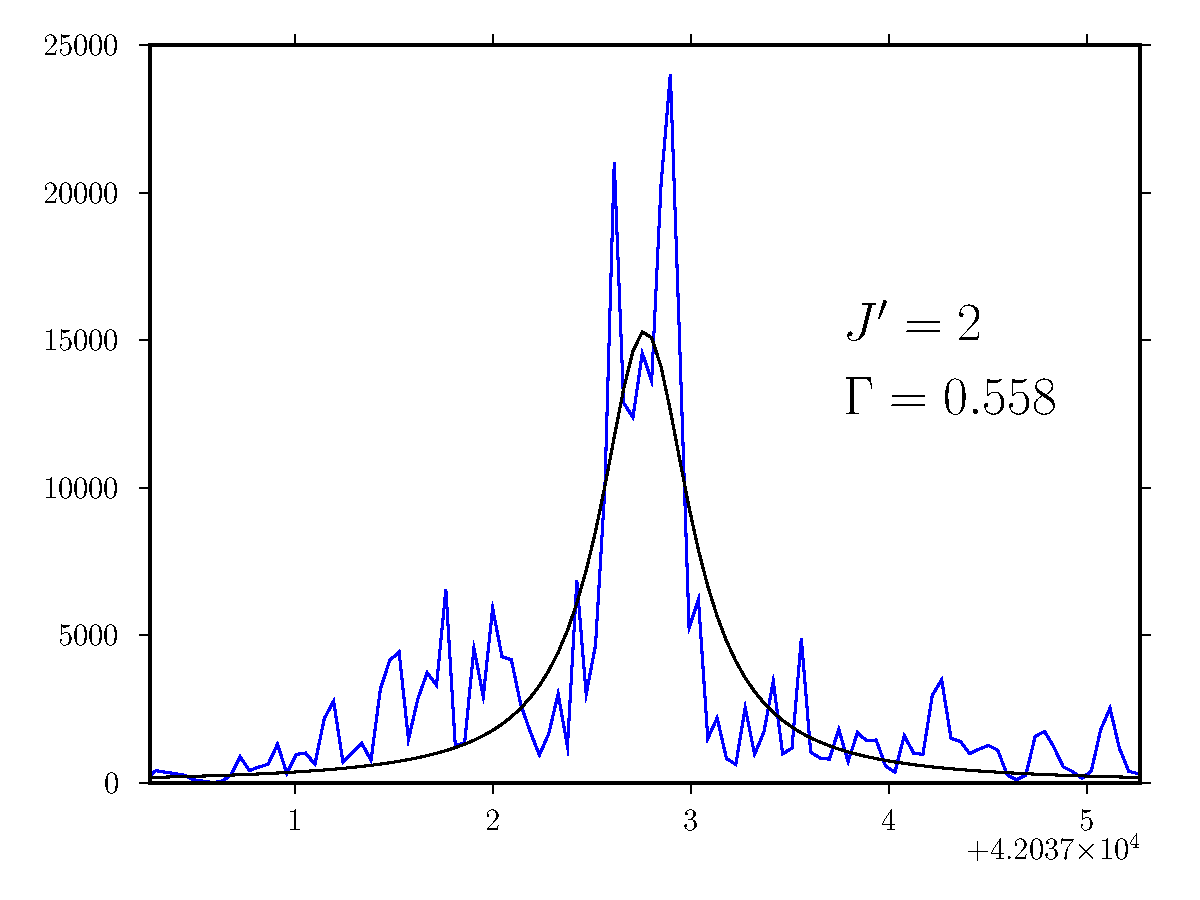
\includegraphics[width=3.2in]{3361-q2-seelemfit}
  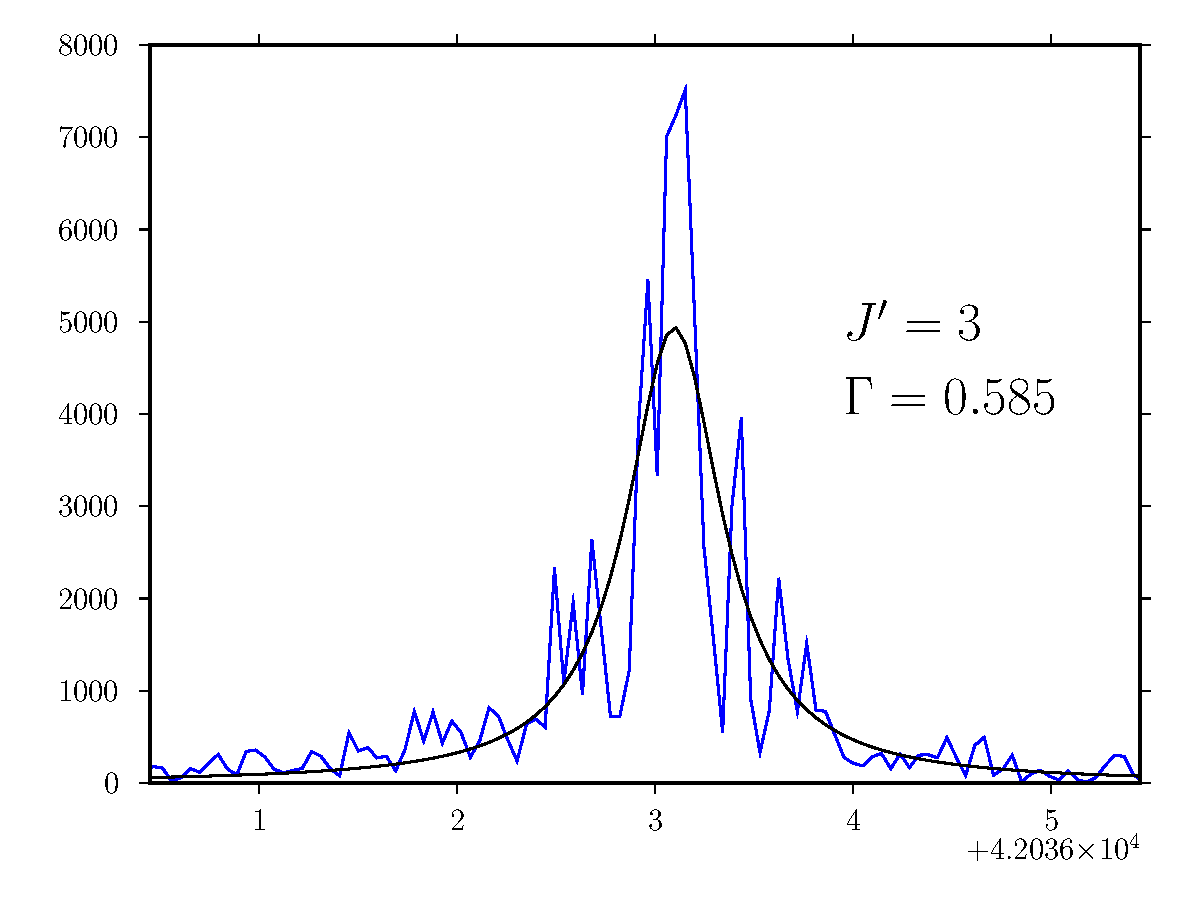
\includegraphics[width=3.2in]{3361-q3-seelemfit}
  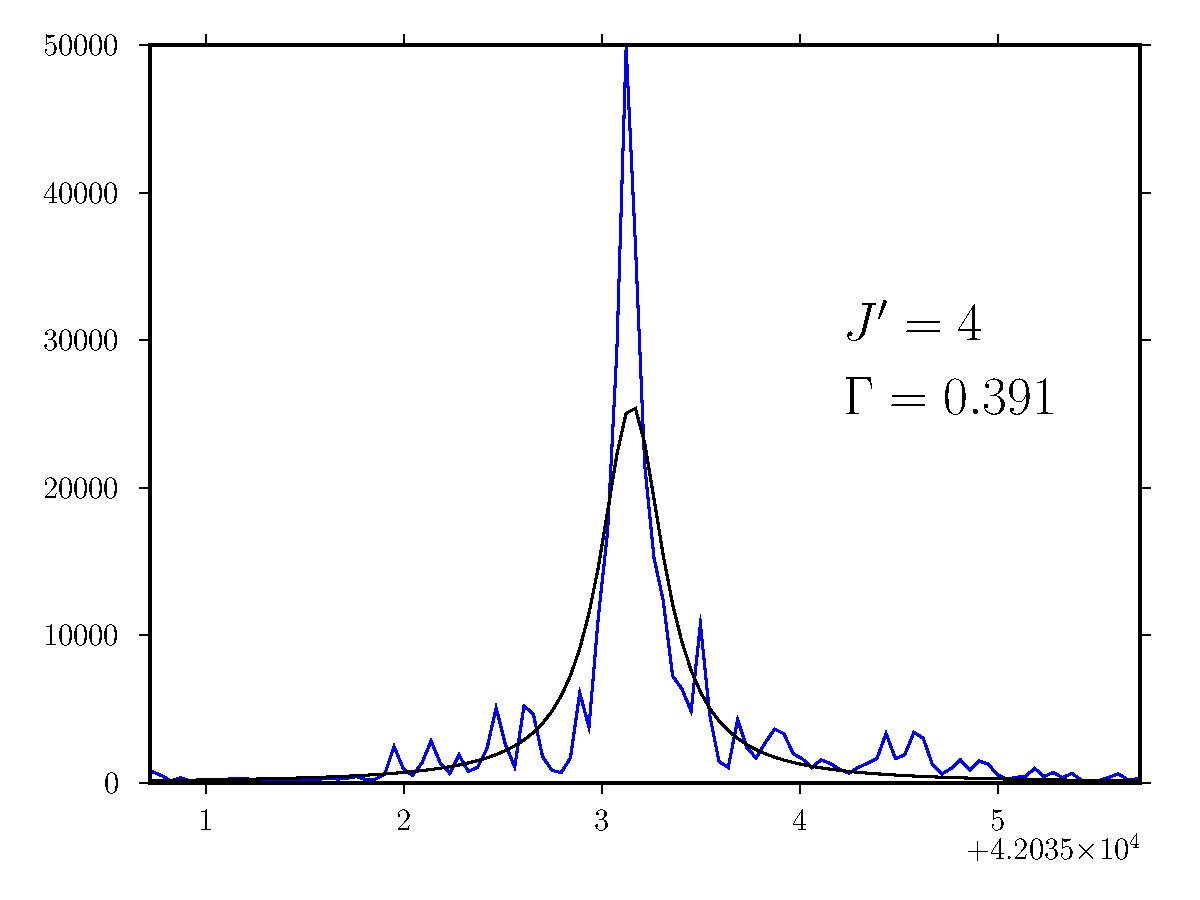
\includegraphics[width=3.2in]{3361-q4-seelemfit}
  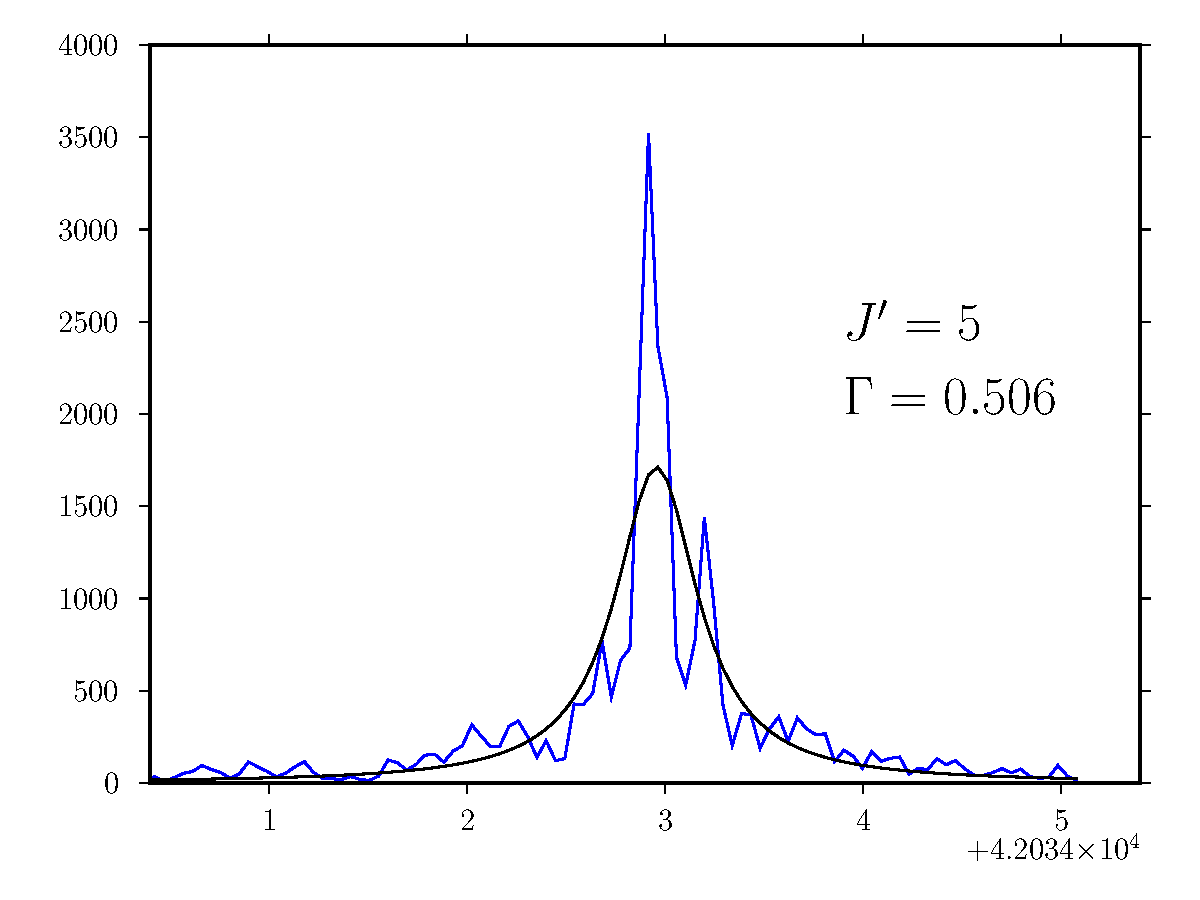
\includegraphics[width=3.2in]{3361-q5-seelemfit}
\end{figure}

%%%%%%%%%%%%%%%%%%%%%%%%%%%%%%%%%%%%%%%%%%%%%%%%%%%%%%
%%
%% END SEELEM FIT FIGURES
%%
%%%%%%%%%%%%%%%%%%%%%%%%%%%%%%%%%%%%%%%%%%%%%%%%%%%%%%

To further examine the properties of the local manifold of nominal
$T_{1,2}$ eigenstates, a modified reduced term value plot is prepared
for the $3^36^1$ \Ka{0} level of $S_1$ acetylene.  To construct this
plot, $S_1$ basis state rotational energies were approximated from the
intensity-weighted center of gravity of the early LIF spectrum.  The
total energy of each state was reduced by an approximate rotational
term energy, $1.04 \: J'(J'+1)$.  The resultant $S_1$ rotational
energies are shown as large square markers in Figure \ref{fig:unfold}.
The energies of nominal triplet $T_{1,2}$ levels observed in the
SEELEM spectrum are shown in the plot with small markers.

For each SEELEM transition, a horizontal bar denotes the approximate
magnitude of the matrix element $H_{\ell m}$, according to equation
\ref{eq:approx-hlm}.  The total magnitude of the horizontal bars is
normalized separately at each value of $J'$.  The energy spacing and
matrix elements show a remarkable uniformity, in agreement with our
proposed simple model for the $T_3 \sim T_{1,2}$ interactions.  The
conclusions drawn from such a figure should be treated with caution,
however, because nominal $T_{1,2}$ states with small matrix elements
may be obscured by others with strong intensity in the SEELEM
spectrum.  Without a better idea of the intrinsic $T_3 \sim T_{1,2}$
dynamics, we have no way of knowing what lurks beneath the lines in
our SEELEM spectra.

Three dotted lines are superimposed on the figure to serve as guides
for the approximate rotational energy dependence of the three spin
components $F_1$, $F_2$, and $F_3$.  The reduced term energies of the
three triplet components have slopes of approximately $-2B$, 0, and
$+2B$ when plotted against $J'$ (not $J'(J'+1)$).  For a $K_T=1$
sublevel, any of the three components may appear, while for a $K_T=0$
sublevel, spin-orbit mixing is allowed only with the $F_1$ or $F_3$
components.  The absence of any apparent rotational structure in the
ensemble of SEELEM-detectable states justifies our statistical
treatment of $T_3 \sim T_{1,2}$ mixing.  The reader is challenged to
find any series of SEELEM detectable states that fit unambiguously to
the slope of the dotted lines.

%%%%%%%%%%%%%%%%%%%%%%%%%%%%%%%%%%%%%%%%%%%%%%%%%%%%%%
%%
%% INSERT UNFOLDED INTENSITY FIGURE
%%
%%%%%%%%%%%%%%%%%%%%%%%%%%%%%%%%%%%%%%%%%%%%%%%%%%%%%%

\begin{figure}
  \caption{Modified reduced term value plot for the $3^36^1$ \Ka{0}
    level of $S_1$ acetylene.  An approximate term energy $1.04 \;
    J'(J'+1)$ is subrtacted from the total $S_1$ rotational energies
    (large markers) and the energies of nominal triplet eigenstates
    observed in the SEELEM spectrum (small markers).  For each
    SEELEM-detectable state, a horizontal bar denotes the relative
    magnitude of the spin-orbit matrix element $H_{\ell m}$.  The
    width of the horizontal bars is normalized separately for each
    value of $J'$.  The energy spacing and matrix elements show a
    remarkable uniformity, which is expected from an extensively mixed
    manifold of $T_{1,2}$ levels.}
  \label{fig:unfold}
  \centering
  \vspace{15mm}
  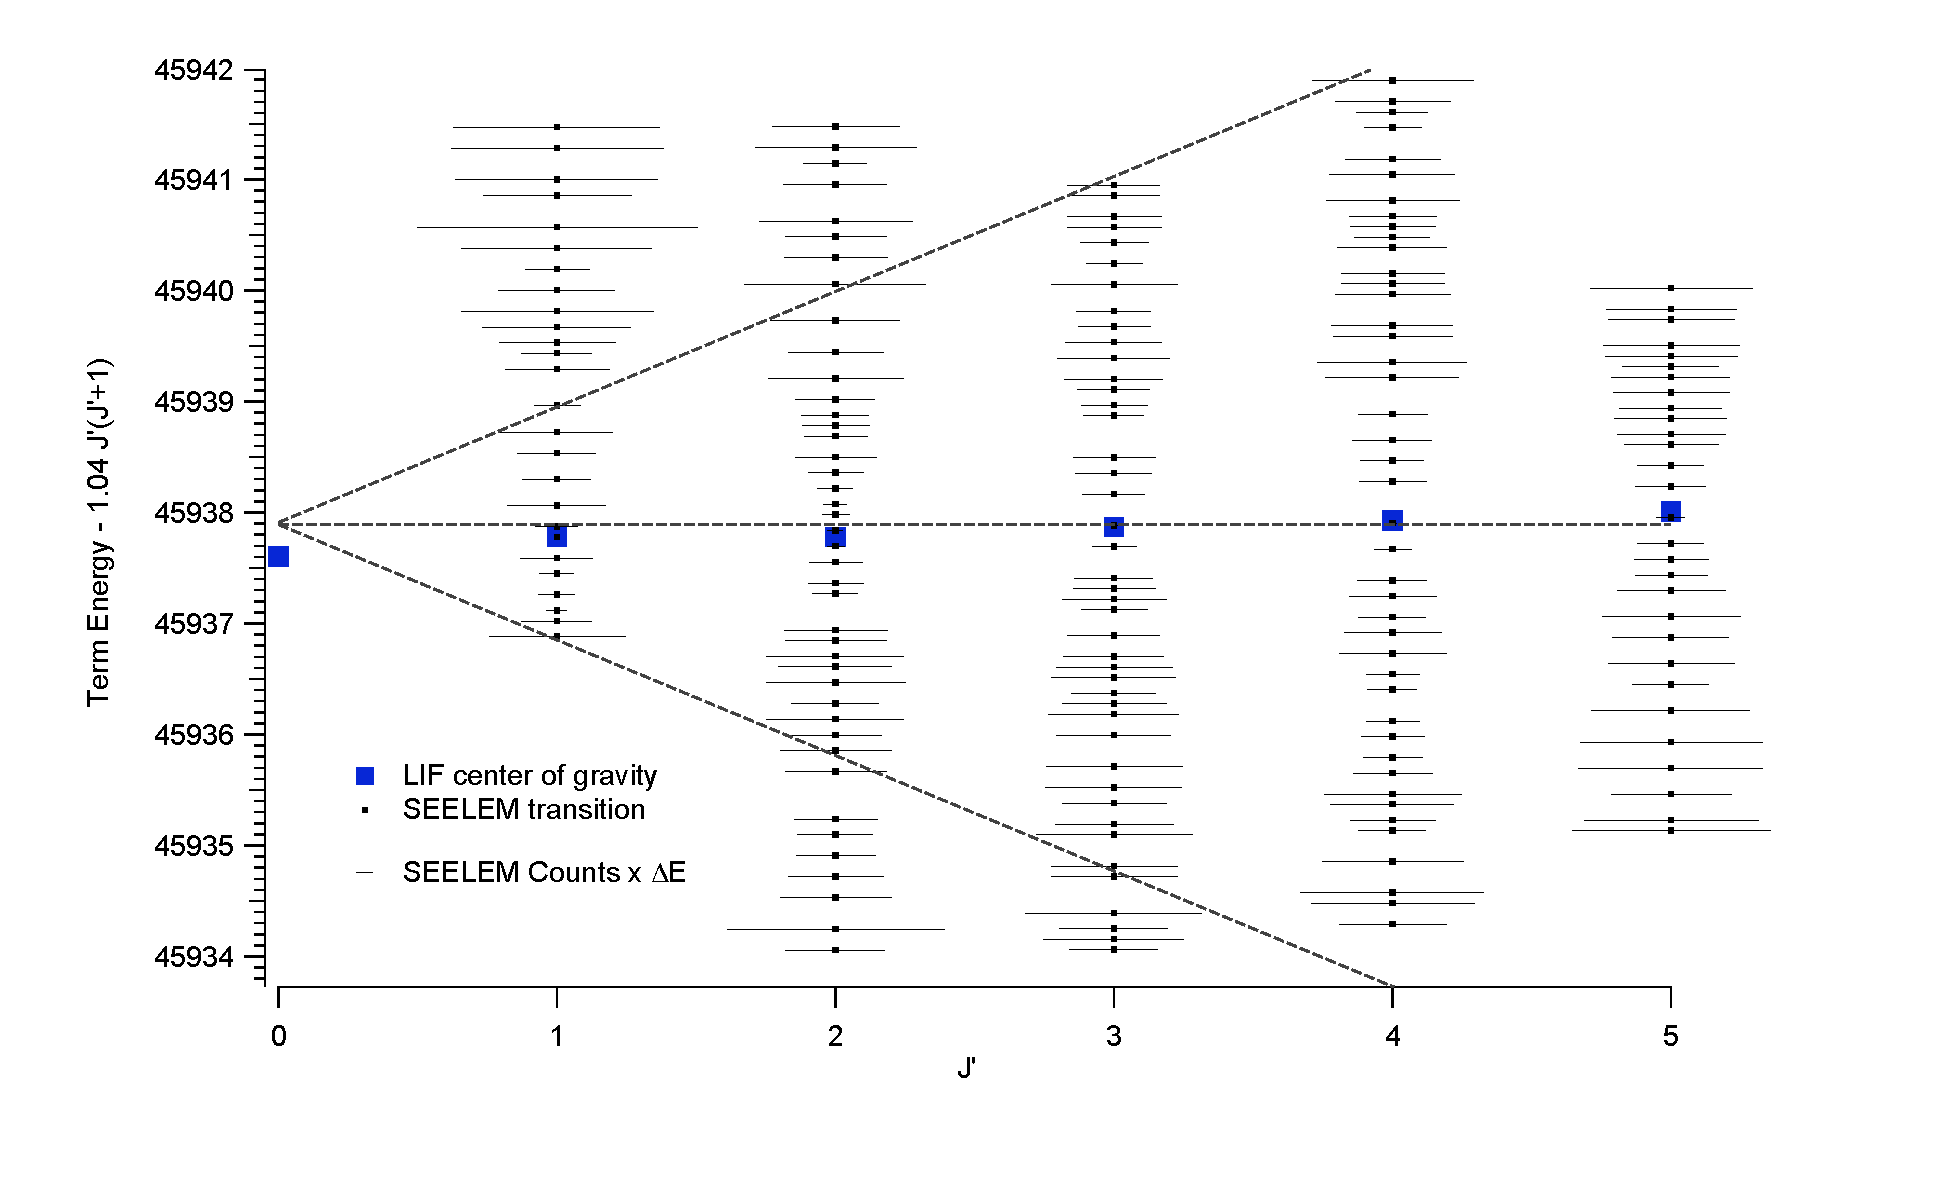
\includegraphics[width=7in, trim=10mm 0mm 50mm 0mm, angle=90]{redterms-3361-unfolded}
\end{figure}

%%%%%%%%%%%%%%%%%%%%%%%%%%%%%%%%%%%%%%%%%%%%%%%%%%%%%%
%%
%% END UNFOLDED INTENSITY FIGURE
%%
%%%%%%%%%%%%%%%%%%%%%%%%%%%%%%%%%%%%%%%%%%%%%%%%%%%%%%

The observation of a $J'=0$ rotational level in $3^36^1$ \Ka{0}
affords us a unique opportunity to estimate the local triplet level
density.  For a triplet vibrational sublevel with $K_T=0$ or $1$, only
a single spin component, $F_3$, is present to mix with a $J'=0$
singlet.  The vibrational symmetry of the triplet is restricted
($\Gamma_T=b$) when $K_T=0$, but unrestricted when $K_T=1$
($\Gamma_T=a$ or $b$), thus we expect to observe that the ratio of
$K_T=1$ sublevels to $K_T=0$ sublevels is 2:1.  (If Coriolis-induced
mixing is complete within the manifold of $T_{1,2}$ levels, the ratio
becomes 1:1, and the state density is decreased by approximately
24\%.)  Over an energy range of approximately 5 \rcm, we observe
approximately 26 total lines in the SEELEM and LIF spectrum.  Of
these, one must be subtracted as the nominal $S_1$ bright state.  The
25 lines that remain are partitioned among triplets with $K_T=0$ and
$1$.  Counting only the expected fraction of those with $K_T=1$, we
are left with 16.6 levels over a range of 5 \rcm, or an observed
triplet level density of $\rho_{T_{1,2}} = 3.3$ per \rcm.  The triplet
level density inferred from this observation is in general agreement
with the high-resolution results of Drabbels and coworkers, who
inferred a level density of approximately 4.9 per \rcm\ from the
highly fractionated LIF spectrum of the $3^3$ \Ka{1} and $3^4$ \Ka{1}
sublevels \cite{drabbels94}.  In their observations, any of the three
spin components of a triplet sublevel with either $K_T=0, 1$ or $2$
may appear in the spectrum.  It is natural that their triplet level
count should be slightly higher and somewhat more uncertain than ours.

% \POINT{Present energy levels and reduced term value plot for $3^36^1$.
%   (See p.97 of 4/2007--8/2007 notebook.)} 

% \POINT{Use $\Delta_3$ statistic, $\Sigma^2$ statistic, or Fourier
%   transform methods? (See p.65 in 11/2007--1/2008 notebook.)}


















\section{Discussion}

The SEELEM and LIF spectra of two acetylene $S_1$ sublevels, $3^36^1$
\Ka{0} and $3^34^1$ \Ka{0}, are compared in order to address the
effects of the non-symmetric bending vibrations, $\nu_4$ and $\nu_6$,
on $S_1 \sim T_3$ vibrational overlap integrals.  The sublevel
involving torsional motion, $3^34^1$ \Ka{0}, is found to have
triplet-induced line splittings on same order of magnitude as the
sublevel involving the antisymmetric in-plane bending motion, $3^36^1$
\Ka{0}.  This result is in contrast to other experimental observations
involving the two motions, which have found perturbations only in
levels involving $\nu_6$ \cite{mizoguchi00, yamakita01}.  A
measurement of the spectral variance is used to place a lower bound on
the $S_1 \sim T_3$ doorway state matrix element.  A lower bound of
approximately 0.1 \rcm\ is obtained for both sublevels.  To be
consistent with the required energy separation of a distant doorway
level from the singlet, the actual $S_1 \sim T_3$ matrix element must
be larger than this lower bound.

To address the identity of $T_3$ vibrational sublevels responsible for
mediating the $S_1 \sim T_{1,2}$ mixing, we thoroughly considered the
vibronic and rotational selection rules for spin-orbit perturbations
in acteylene.  A calculation of vibrational overlap integrals between
$S_1$ and $T_3$, based on recent \emph{ab initio} calculations of the
potential energy surfaces, reveals a propensity for particular
vibrational modes of $T_3$ to promote overlap with $S_1 \:\; 3\nu_3 +
\nu_4$ and $3\nu_3 + \nu_6$.  The $T_3$ \emph{trans}-bending
vibration ($\nu_4$) and torsional vibration ($\nu_2$) are found to
increase vibrational overlap with $S_1 \:\; 3\nu_3 + \nu_4$, while a
combination of the $T_3$ \emph{trans} and \emph{cis}-bending ($\nu_6$)
vibrations is observed to increase vibrational overlap with $S_1 \:\;
3\nu_3 + \nu_6$.

In terms of vibrational overlap and spin-orbit mixing, two questions
must be addressed: where are the relevant stationary phase points at
which the vibrational overlap integrals accumulate, and are the
electronic seams of intersection accessible at these points?  We first
consider the $S_1 \:\; 3\nu_3 + \nu_6$ level.  It has been suggested
in the literature that $S_1 \sim T_3$ vibrational overlap may
accumulate at a half-linear turning point geometry \cite{mizoguchi00}.
Recent calculations carried out by Josh Baraban indicate that the $S_1
\;\; 3\nu_3 + \nu_6$ level has appreciable amplitude in this region of
phase space, particularly in comparison to the $S_1 \;\; 3\nu_3$ level
\cite{baraban08}.  The calculation of vibrational overlap integrals
indicates a similar picture for the $T_3$ surface, where the critical
half-linear geometry is accessible a combination of the $T_3$
\emph{trans} ($\nu_4$) and \emph{cis}-bending ($\nu_6$) vibrations.
The region of $S_1 \sim T_3$ electronic intersection is also
accessible to wavefunctions with amplitude in a half-linear geometry.
The calculations of Ventura and coworkers indicate that the seam of
$S_1 \sim T_3$ intersection passes through the half-linear region of
phase space at a CCH bending angle of approximately 140\degrees\ (see
their figure 5b) \cite{ventura03}.  We conclude that our explanation
for the $T_3$ perturbations in $S_1 \;\; 3^36^1$ \Ka{0} is in accord
with previous research.

The characterization of stationary phase points for the $S_1 \:\;
3\nu_3 + \nu_4$ level is more of a challenge.  Calculated
wavefunctions for $S_1$ are not available along the torsional
coordinate.  However, our calculations of $T_3$ vibrational overlap
integrals supports the general Franck-Condon argument that excitation
in the $T_3$ \emph{trans}-bending vibration ($\nu_4$) and torsional
vibration ($\nu_2$) increase the magnitude of vibrational overlap.
However, the seam of $S_1 \sim T_3$ intersection is generally
inaccessible along the torsional coordinate.  The \emph{ab initio}
calculations of Ventura and coworkers predict that the $S_1 \sim T_3$
seam of intersection in the torsional coordinate occurs on the
\textbf{opposite side} of the torsional well from $S_1$ (see their
Figure 6), at angles between 90 and 140 \degrees\ \cite{ventura03}.
The seam of intersection is most accessible along the torsional
coordinate at near-linear geometries.  It should also be noted
that the seam of intersection is located at lower energies along the
torsional coordinate.

One possible explanation for the observed mixing in $3^34^1$ \Ka{0}
is that this sublevel gains $T_3$ character through $b$-axis Coriolis
coupling with the \Ka{1} sublevel of $3^36^1$ \Ka{1}.  The $3^36^1$
\Ka{1} is known to be strongly perturbed by a level of $T_3$.  The
matrix element for $b$-axis Coriolis interaction between $3^34^1$
\Ka{0} and $3^36^1$ \Ka{1} is approximately 1.4 \rcm.  The energy
separation between the $3^34^1$ \Ka{0} level and the $3^36^1$ \Ka{1}
sublevel is approximately 42 \rcm.  This leads to a mixing angle of
about 0.03.  The observed splitting in $3^36^1$ \Ka{1} is
approximately 1 \rcm, indicating what is probably a local $T_3$
perturber with a matrix element of 0.5 \rcm.  Coriolis mixing with
$3^36^1$ \Ka{1} would lead to a second-order spin-orbit interaction
with the $T_3$ perturber on the order of $0.5 \times 0.03 = 0.015$
\rcm, which is not sufficient to satisfy the lower bound condition of
0.1 \rcm for the $S_1 \sim T_3$ matrix element.  The observed
spin-orbit matrix element for $3^34^1$ \Ka{0} cannot be attributed to
mixing with the $3^36^1$ \Ka{1} sublevel.

% \TODO{Examine observations in terms of Josh's new acetylene
%   wavefunction calculations.  The $\nu_3 \sim \nu_6$ anharmonic matrix
%   element is much larger than the $\nu_3 \sim \nu_4$ matrix element,
%   and provides a pathway for $T_{2,1} \leftarrow T_3 \leftarrow S_1$
%   coupling.  IF the stationary phase point is in a half-linear
%   geometry, the combination of modes 3 and 6 is the perfect storm to
%   drive a node of the vibrational wavefunction in the right direction.
%   Due to the nature of the potential well, wavefunctions with
%   trans-vibration alone spread out at a 45\degrees angle to the
%   stationary phase point.  One node of cis-bend is enough to ``push''
%   a node of the wavefunction directly toward the half-linear turning
%   point. }

% \TODO{Do we see too many doorways, or do we observe the expected
%   number?  The answer lies in the definition of a doorway state -- it
%   is simply that level of $T_3$ with the largest mixing
%   angle. Reiterate that we basically are working with a three tier
%   model in the limit of low level density in the second tier.  The
%   doorway model is a natural consequence of operating in this limit,
%   because energy denominator effects make it likely that a single
%   $T_3$ level mixes to a much greater degree than all others.
%   However, there is no fundamental principle which precludes
%   interaction with more than one doorway.  A single doorway model is
%   simply our zero-order picture.}

The technique of IR-UV double resonance excitation allows, in contrast
to previous one-photon studies, the observation of the full SEELEM
intensity envelope surrounding each rovibronic transition in an $S_1$
sublevel.  The cluster of nominal $T_{1,2}$ eigenstates appearing in
the spectrum is fit to a Lorentzian distribution, following a simple
statistical coupling model.  The product $\alpha H_{\ell m}$ is
determined by the fit results to be on the order of 0.1 \rcm.  

% Since
% the mixing amplitude $\alpha$ is certainly less than 0.7, the $T_3 \sim
% T_{1,2}$ matrix element must be at least 0.14

One may ask: do we observe \emph{too many} doorway states in the
spectrum of \ce{C2H2}?  The answer lies in the definition of a doorway
state, and is inherent to the doorway model.  The doorway model is
based on the more general tier model of energy levels
\cite{stuchebrukhov93a, stuchebrukhov93b}.  In the zeroth tier is the
bright state, the $S_1$ sublevel assigned in the LIF spectrum.  The
first tier contains the vibrational sublevels of $T_3$, and the second
contains sublevels of $T_{1,2}$.  The tier model simplifies to the
doorway model in the limit of small level density in the first tier.
In this limit, the effect of energy denominators is to select, in most
cases, one state of $T_3$ with the largest matrix element at the
nearest energy to dominate the mixing.  However, there is nothing
inherent to the model that prevents more than one doorway from being
active for a particular $S_1$ vibrational level.  Our zero-order
assumption of a single doorway is based only on a propensity that
results from the effects of energy denominators and the local density
of $T_3$ levels.  The nature of the doorway model also ``guarantees''
a doorway state for any $S_1$ level for which weak $S_1 \sim T_{1,2}$
mixing is observed.  The $S_1 \sim T_3$ matrix element may be small in
comparison to other $S_1$ levels, but $S_1 \sim T_{1,2}$ is still
mediated by level of $T_3$ with the largest ratio
$H_{s\ell}/\Delta E_{s\ell}$.

It is the stated goal of this research project to observe an acetylene
$T_3$ level ``in the wild,'' that is, at an energy separation of more
than 2 \rcm\ from the $S_1$ level from which it borrows intensity.  To
date, this goal remains elusive.  We speculate here on the prospects
for direct observation of a lone $T_3$ level, in light of our current
results.
\begin{enumerate}
\item A $T_3$ doorway state is fractionated among the manifold of
  $T_{1,2}$ levels with a full width of $2 \pi (1-\alpha^2)^2 H_{\ell
    m} \rho_m$.  An accurate determination of the average $T_3 \sim
  T_{1,2}$ matrix element is therefore crucial for the esimation of
  this width.
\item The primary interaction for a distant $T_3$ doorway state is via
  the $F_1$ or $F_3$ spin components.  The term energy of these
  components changes by approximately $\pm 2$ \rcm\ per $J'$, causing
  consecutive rotational transitions to be widely spaced in frequency.
\end{enumerate}
The prospect of roecording weak, highly fractionated transitions over
large frequency ranges seems daunting.  An accurate estimate of the
average $T_3 \sim T_{1,2}$ matrix element would allow the
experimentalist an appropriate frequency step size to use in a search
for a lone $T_3$ level.  The average $T_3 \sim T_{1,2}$ matrix element
also determines the maximum intensity of the transition to the $T_3$
level, since the maximum value Lorentzian intensity is inversely
proportional to the spectral width.


% \section{Conclusion}

% \TODO{Write this section.}


% \bibliography{master}
% \bibliographystyle{plain}
% \end{document}
% LocalWords:  sublevel initio Condon Mizoguchi Zeeman sublevels Yamakita Cui
% LocalWords:  publised Morokuma deperturbation
